% =============================================================================
%  Capítulo 5: Optimización no suave y global
%  Basado en:
%    Steven L. Brunton, "Optimization: A Bootcamp for Machine Learning,
%    Inverse Problems, and Control", Cambridge University Press, 2026.
%    Capítulo 5, secciones 5.1--5.5 (pp. 167--202).
%
%  Compilar:  make
% =============================================================================

\documentclass[10pt,aspectratio=169]{beamer}

% --- Idioma y codificación ---------------------------------------------------
\usepackage[utf8]{inputenc}
\usepackage[T1]{fontenc}
\usepackage[spanish,es-nodecimaldot]{babel}

% --- Matemáticas -------------------------------------------------------------
\usepackage{amsmath,amssymb,mathtools}

% --- Tablas, figuras y código -------------------------------------------------
\usepackage{booktabs}
\usepackage{tabularx}
\usepackage{array}
\usepackage{lmodern}
\usepackage{microtype}
\usepackage{graphicx}
\usepackage{listings}
\usepackage{xcolor}

% --- Colores -----------------------------------------------------------------
\definecolor{unah}{RGB}{0,82,155}
\definecolor{acento}{RGB}{0,135,110}
\definecolor{alerta}{RGB}{180,75,45}
\definecolor{claro}{RGB}{235,244,250}

\setbeamercolor{structure}{fg=unah}
\setbeamercolor{frametitle}{fg=unah}
\setbeamercolor{itemize item}{fg=acento}
\setbeamercolor{itemize subitem}{fg=unah}
\setbeamercolor{block title}{fg=white,bg=unah}
\setbeamercolor{block body}{bg=claro}
\setbeamertemplate{itemize item}{\color{acento}\scriptsize$\blacktriangleright$}
\setbeamertemplate{itemize subitem}{\color{unah}\scriptsize$\bullet$}
\setbeamertemplate{blocks}[rounded][shadow=false]

% --- Plantillas --------------------------------------------------------------
\setbeamertemplate{navigation symbols}{}
\setbeamertemplate{footline}[frame number]
\setbeamersize{text margin left=7mm,text margin right=7mm}

% --- Atajos ------------------------------------------------------------------
\newcommand{\fuente}{\vfill{\scriptsize\color{gray}Brunton, \emph{Optimization Bootcamp}, Cap.~5}}
\newcommand{\R}{\mathbb{R}}
\newcommand{\norm}[1]{\left\lVert #1 \right\rVert}
\newcommand{\prox}{\operatorname{prox}}
\newcommand{\proj}{\operatorname{proj}}
\newcommand{\argmin}{\operatorname*{arg\,min}}
\newcommand{\sign}{\operatorname{sign}}
\newcommand{\ind}{\mathbf{1}}

\lstdefinestyle{pythontiny}{
  language=Python,
  basicstyle=\ttfamily\tiny,
  keywordstyle=\color{acento}\bfseries,
  commentstyle=\color{gray},
  stringstyle=\color{alerta},
  showstringspaces=false,
  columns=fullflexible,
  keepspaces=true,
  frame=single,
  rulecolor=\color{unah!35},
  backgroundcolor=\color{gray!4},
  breaklines=true,
  tabsize=4
}

\lstdefinestyle{python}{
  language=Python,
  basicstyle=\ttfamily\scriptsize,
  keywordstyle=\color{acento}\bfseries,
  commentstyle=\color{gray},
  stringstyle=\color{alerta},
  showstringspaces=false,
  columns=fullflexible,
  keepspaces=true,
  frame=single,
  rulecolor=\color{unah!35},
  backgroundcolor=\color{gray!4},
  breaklines=true,
  tabsize=4
}

\title{Cap. 5: Optimización No Suave y Global}
\subtitle{Gradiente proximal, búsqueda sin derivadas y algoritmos evolutivos}
\author{Luis Berlioz}
\date{\today}

% =============================================================================
\begin{document}
% =============================================================================

\begin{frame}
  \titlepage
\end{frame}

\begin{frame}{Ruta del capítulo}
  \small
  \begin{columns}[T,onlytextwidth]
    \begin{column}{.48\textwidth}
      \tableofcontents
    \end{column}
    \begin{column}{.48\textwidth}
      \begin{block}{Pregunta guía}
        \small
        ¿Cómo se optimiza cuando el objetivo no tiene gradiente útil, o cuando
        la geometría es no convexa?
      \end{block}
      \vspace{2mm}
      \begin{itemize}
        \item \textbf{Con estructura}: optimización convexa y proximal.
        \item \textbf{Sin estructura}: búsqueda sin derivadas.
        \item \textbf{Con población}: búsqueda distribuida y por enjambre.
      \end{itemize}
      \vspace{2mm}
      {\footnotesize\color{gray}
       El libro advierte: este capítulo tiene ``un poco menos de estructura que
       los anteriores'', porque la optimización no convexa es ella misma menos
       estructurada.}
    \end{column}
  \end{columns}
\end{frame}

\begin{frame}{El problema en una línea}
  \small
  \[
    \min_x\; f(x) + g(x) \tag{5.1}
  \]
  \begin{columns}[T,onlytextwidth]
    \begin{column}{.48\textwidth}
      \begin{itemize}
        \item $f$: suave (típicamente convexa, gradiente Lipschitz continuo).
        \item $g$: posiblemente no suave (típicamente convexa): $\norm{x}_1$,
          norma nuclear, variación total.
        \item El descenso de gradiente del Cap.~2 \textbf{no aplica} cuando $g$
          es no suave.
      \end{itemize}
    \end{column}
    \begin{column}{.48\textwidth}
      \begin{itemize}
        \item El Cap.~4 ya tenía el par $\norm{Ax-b}_2^2 + \lambda\norm{x}_1$
          (LASSO): ahora se resuelve \emph{sin} derivar una fórmula cerrada.
        \item El operador proximal reaparece en el Cap.~6 con ADMM.
      \end{itemize}
    \end{column}
  \end{columns}
  \begin{block}{La cadena del capítulo}
    \centering\scriptsize
    gradiente proximal $\to$ umbralización $\to$ restricciones y proyección
    $\to$ separación de variables y SR3 $\to$ búsqueda sin derivadas
    $\to$ recocido simulado $\to$ algoritmos evolutivos $\to$ enjambre
  \end{block}
\end{frame}

\begin{frame}{Panel 5.1: la hegemonía convexa se relativiza}
  \small
  \begin{columns}[T,onlytextwidth]
    \begin{column}{.48\textwidth}
      \begin{block}{Hasta los 90}
        \small
        Tras el simplex de Dantzig, la convexidad fue la propiedad que
        garantizaba la tratabilidad: mínimos locales $=$ globales, y una
        potente teoría de dualidad (Rockafellar, 1970).
      \end{block}
      \begin{block}{Hoy}
        \small
        Los métodos de separación y proximales, y el éxito del aprendizaje
        profundo hicieron mainstream la no convexidad. La optimización convexa sigue
        siendo fundacional, pero ya no es la única plantilla.
      \end{block}
    \end{column}
    \begin{column}{.48\textwidth}
      \begin{itemize}
        \item \textbf{Lo que no cambió}: la convexidad sigue siendo la
          referencia; los algoritmos de primer orden que la usan siguen
          siendo los más formales.
        \item \textbf{Lo que cambió}: la no convexidad dejó de ser un
          callejón sin salida matemático y pasó a ser una herramienta
          legítima.
      \end{itemize}
      \vspace{2mm}
      {\footnotesize\color{gray}
       Panel 5.1, p.~168.}
    \end{column}
  \end{columns}
\end{frame}

\begin{frame}{Panel 5.2: multiobjectivo y frente de Pareto}
  \small
  \[
    f(x) = \norm{Ax-b}_2^2 + \lambda\norm{x}_0
  \]
  \begin{itemize}
    \item Para un $\lambda$ fijo: un único objetivo escalar. Pero a menudo
      interesan los \textbf{tradeoffs} entre varios pesos $\lambda$.
    \item Barrer $\lambda$ produce la familia Pareto; el \textbf{frente de
      Pareto} son las soluciones donde mejorar un objetivo empeora otro.
    \item Útil en diseño cuando el peso de los términos no está decidido.
  \end{itemize}
  \begin{block}{Los saltos del frente señalan buenos $\lambda$}
    \small
    En ajuste de modelos, un salto en la curva de Pareto suele marcar el
    punto donde empieza el \emph{overfitting}. Si hay datos de prueba, se
    valida sobre ellos; si no, los saltos son la única señal.
  \end{block}
  \fuente
\end{frame}

% =============================================================================
\section{Gradiente proximal}
% =============================================================================

\begin{frame}{La idea: sustituir el paso de gradiente}
  \small
  \begin{columns}[T,onlytextwidth]
    \begin{column}{.48\textwidth}
      \begin{itemize}
        \item En vez de derivar la solución de $f+g$, se \textbf{define} un
          operador que incorpora el término no suave.
        \item Alterna: un paso de gradiente sobre la parte suave $f$, y un
          paso \emph{proximal} sobre el regularizador $g$.
        \item Ya se conoce el prox de \emph{docenas} de regularizadores
          comunes: se sustituye directamente por el paso de gradiente.
      \end{itemize}
    \end{column}
    \begin{column}{.48\textwidth}
      \begin{block}{R5.1 --- El operador proximal (p.~170)}
        \small
        \[
          \prox_{\gamma,g}(z) := \argmin_x\;
          \tfrac{1}{2}\norm{x-z}_2^2 + \gamma g(x) \tag{5.3}
        \]
        El subíndice $\gamma$ es explícito: el operador depende del paso del
        problema \emph{sin} regularizar y de $g$.
      \end{block}
      \begin{block}{R5.2 --- El paso proximal (p.~170)}
        \small
        \[
          x_{k+1} = \prox_{\gamma,g}\!\left(x_k - \gamma\nabla f(x_k)\right)
          \tag{5.2}
        \]
        con $z = x_k - \gamma\nabla f(x_k)$.
      \end{block}
    \end{column}
  \end{columns}
\end{frame}

\begin{frame}{R5.3 --- La envolvente de Moreau}
  \small
  Se asume $f$ convexa con gradiente Lipschitz continuo:
  \[
    f(x) \le f(x_0) + (x-x_0)^T\nabla f(x_0)
    + \tfrac{\beta}{2}\norm{x-x_0}_2^2 \tag{5.4a}
  \]
  Completando el cuadrado:
  \[
    \begin{aligned}
    = f(x_0) &+ \tfrac{\beta}{2}\norm{x - \left(x_0 - \tfrac{1}{\beta}\nabla f(x_0)\right)}_2^2
    - \tfrac{1}{2\beta}\norm{\nabla f(x_0)}_2^2 \;\equiv\; m_0(x)
    \end{aligned} \tag{5.4b}
  \]
  \begin{itemize}
    \item Sólo el término central depende de $x$: minimizar $m_0$ equivale a
      $x = x_0 - \tfrac{1}{\beta}\nabla f(x_0)$, es decir, \textbf{descenso de
      gradiente con $\gamma = 1/\beta$}.
    \item Ese paso sale de un método de Newton sobre la cuadrática envolvente
      de curvatura $\beta/2$ --- y puede ser \emph{bastante ineficiente}: por
      eso conviene una búsqueda lineal.
  \end{itemize}
  \fuente
\end{frame}

\begin{frame}{R5.4 --- El proximal gradient como argmin}
  \small
  Añadiendo $g$ a (5.4a):
  \[
    f(x)+g(x) \le f(x_0) + (x-x_0)^T\nabla f(x_0)
    + \tfrac{\beta}{2}\norm{x-x_0}_2^2 + g(x) \tag{5.5a}
  \]
  \[
    \begin{aligned}
    = f(x_0) &+ \tfrac{\beta}{2}\norm{x - \left(x_0 - \tfrac{1}{\beta}\nabla f(x_0)\right)}_2^2
    - \tfrac{1}{2\beta}\norm{\nabla f(x_0)}_2^2 + g(x)
    \end{aligned} \tag{5.5b}
  \]
  \begin{block}{R5.4a --- Cota de descenso}
    \small
    \[
      (f+g)(x_1) \le (m_0+g)(x_1) \le (m_0+g)(x_0) = (f+g)(x_0)
    \]
  \end{block}
  \begin{itemize}
    \item El argmin de $m_0(x)+g(x)$ \emph{no} se calculó explícitamente:
      \textbf{es el prox}. En la práctica puede ser difícil.
    \item \textbf{Advertencia}: con $f(x)=\norm{Ax-b}_2^2$, la curvatura
      $\beta/2$ es pesimista $\to$ descenso lento. De ahí SR3 y ADMM (Cap.~6).
  \end{itemize}
  \fuente
\end{frame}

\begin{frame}{E5.1 --- LASSO con gradiente proximal}
  \small
  \textbf{Prox de} $g(x)=\lambda\norm{x}_1$: el objetivo se separa por coordenadas.
  \[
    \prox_{\frac{1}{\beta},\lambda\norm{\cdot}_1}(z)
    = \argmin_x \sum_{j=1}^{n}\Big[\tfrac{\beta}{2}(x_j-z_j)^2 + \lambda|x_j|\Big]
  \]
  \begin{columns}[T,onlytextwidth]
    \begin{column}{.48\textwidth}
      \textbf{Por derivada (caso $x_j>0$):}
      \[
        \beta(x_j-z_j) + \lambda = 0 \;\Longrightarrow\; x_j - z_j = -\tfrac{\lambda}{\beta}
      \]
      \textbf{Rewrite por argumento:} se quiere una condición sobre $z_j$:
      \[
        z_j > \tfrac{\lambda}{\beta} \;\Longrightarrow\; x_j^\ast = z_j - \tfrac{\lambda}{\beta}
      \]
    \end{column}
    \begin{column}{.48\textwidth}
      \begin{block}{R5.5 --- Umbralización suave (soft thresholding)}
        \small
        \[
          x_j^\ast = \sign(z_j)\,\max\Big\{|z_j| - \tfrac{\lambda}{\beta},\, 0\Big\}
        \]
        Umbral $\tau = \lambda/\beta$. Es exactamente \textbf{ISTA}.
        Las variantes aceleradas (FISTA) pasan de $O(1/k)$ a $O(1/k^2)$.
      \end{block}
      \vspace{1mm}
      {\footnotesize\color{gray}pp.~172--173.}
    \end{column}
  \end{columns}
  \fuente
\end{frame}

\begin{frame}{E5.1 --- Figura 5.1: el operador proximal}
  \small
  \begin{center}
    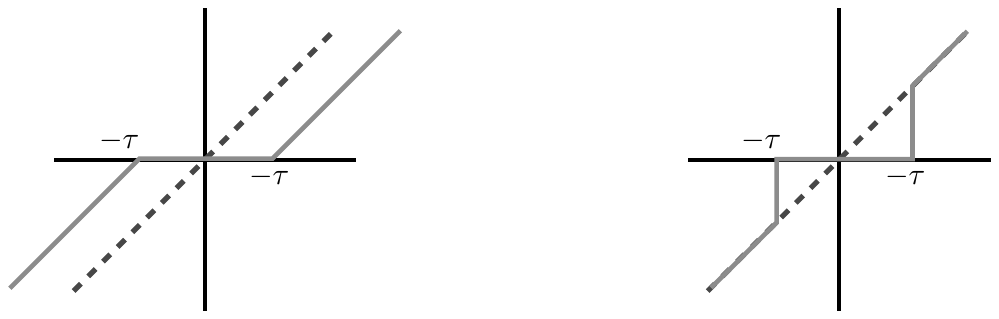
\includegraphics[width=.72\textwidth]{images/fig_5_1.png}
  \end{center}
  \vspace{-2mm}
  {\scriptsize\color{gray}
   Fig.~5.1 (p.~173): operador de gradiente proximal para regresión regularizada
   con $\ell_1$ (izquierda) y $\ell_0$ (derecha). Eje horizontal: la entrada $z_j$;
   eje vertical: la salida $x_j^\ast$.}
  \begin{itemize}
    \item La umbralización suave es una \emph{regresión lineal por morceaux} con
      un único punto de quiebre, en $z_j = \pm\tau$.
  \end{itemize}
  \fuente
\end{frame}

\begin{frame}{E5.2 --- El problema $\ell_0$ con gradiente proximal}
  \small
  \textbf{Prox de} $g(x)=\lambda\norm{x}_0$:
  \[
    \prox_{\frac{1}{\beta},\lambda\norm{\cdot}_0}(z)
    = \argmin_x \sum_{j=1}^{n}\Big[\tfrac{\beta}{2}(x_j-z_j)^2 + \lambda\,\ind(x_j \neq 0)\Big]
  \]
  \begin{columns}[T,onlytextwidth]
    \begin{column}{.48\textwidth}
      \textbf{Aquí no se derivó}: se balancean los dos términos.
      \begin{itemize}
        \item $x_j^\ast = 0$: costo $\tfrac{\beta}{2}z_j^2$.
        \item $x_j^\ast = z_j \neq 0$: costo $\lambda$.
      \end{itemize}
      Se elige el menor de los dos.
    \end{column}
    \begin{column}{.48\textwidth}
      \begin{block}{R5.6 --- Umbralización dura (hard thresholding)}
        \small
        \[
          x_j^\ast = \begin{cases}
            0, & z_j^2 < \tfrac{2\lambda}{\beta}\\[2mm]
            z_j, & z_j^2 > \tfrac{2\lambda}{\beta}
          \end{cases}
        \]
        Umbral $\tau = \sqrt{2\lambda/\beta}$.
      \end{block}
      \vspace{1mm}
      {\footnotesize\color{gray}
       \emph{``El problema $\ell_0$ no es siquiera diferenciable ni continuo,
       y aun así es posible calcular el paso de gradiente proximal.''} (p.~174)}
    \end{column}
  \end{columns}
  \fuente
\end{frame}

\begin{frame}{E5.1 --- Figura 5.2: campos vectoriales del LASSO}
  \small
  \begin{center}
    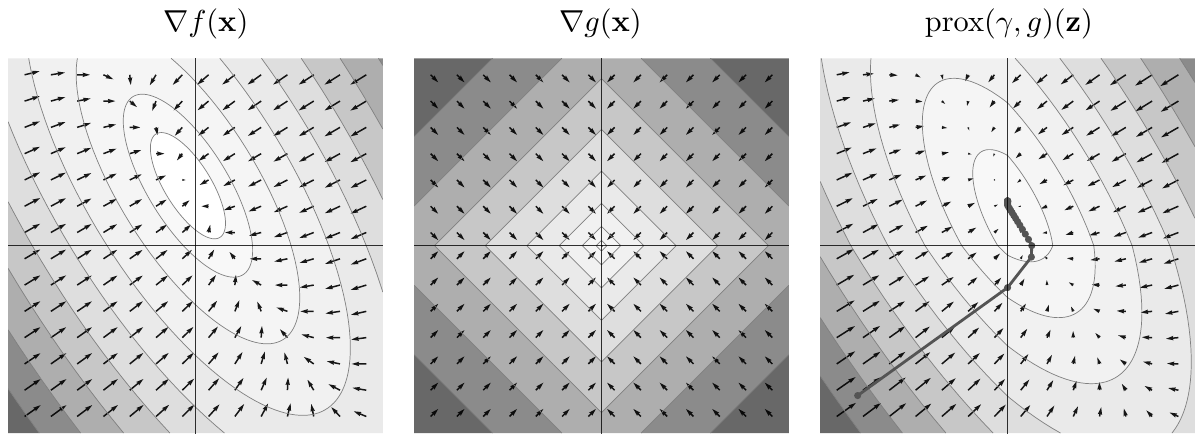
\includegraphics[width=.78\textwidth]{images/fig_5_2.png}
  \end{center}
  \vspace{-2mm}
  {\scriptsize\color{gray}
   Fig.~5.2 (p.~173): campos vectoriales de gradiente y conjuntos de nivel de la
   pérdida para LASSO: (izq.) $f(x)=\norm{Ax-b}_2^2$; (centro) $g(x)=\lambda\norm{x}_1$;
   (der.) campo del gradiente proximal y el descenso proximal por gradiente.}
  \fuente
\end{frame}

\begin{frame}{Restricciones: el indicador y la proyección}
  \small
  \begin{columns}[T,onlytextwidth]
    \begin{column}{.48\textwidth}
      \begin{block}{R5.7 --- Indicador del conjunto factible (p.~174)}
        \small
        \[
          g(x)=\delta_C(x) = \begin{cases}
            0, & x \in C\\
            \infty, & x \notin C
          \end{cases}
        \]
        No suave, discontinua, no acotada. Pero su prox se puede calcular.
      \end{block}
      \begin{block}{R5.8 --- El prox del indicador es la proyección}
        \small
        \[
          \prox_{\frac{1}{\beta},\delta_C}(z)
          = \argmin_{x\in C} \tfrac{\beta}{2}\norm{x-z}_2^2
          \equiv \proj_C(z)
        \]
      \end{block}
    \end{column}
    \begin{column}{.48\textwidth}
      \textbf{R5.9 --- Gradiente proyectado}: iniciar con $x_0\in C$, dar un
      paso de gradiente sin restricciones y \textbf{proyectar de vuelta}:
      \[
        z_{k+1} = x_k - \gamma\nabla f(x_k),
        \qquad x_{k+1} = P_C(z_{k+1})
      \]
      \textbf{R5.10 --- Proyección sobre cajas} (pp.~174--175):
      \begin{align}
        \min_x \tfrac{1}{2}\norm{Ax-b}_2^2 \tag{5.6a}\\
        \text{s.t.}\quad \ell \le x \le u \tag{5.6b}
      \end{align}
      \[
        P_{[\ell,u]}(z)_j = \min\{u_j, \max\{\ell_j, z_j\}\}
      \]
      {\footnotesize\color{gray}
       Los mínimos cuadrados restringidos a caja se revisitan con
       multiplicadores de Lagrange en el Cap.~6.}
    \end{column}
  \end{columns}
  \fuente
\end{frame}

\begin{frame}{Separación de variables (*operator splitting*)}
  \small
  \begin{columns}[T,onlytextwidth]
    \begin{column}{.48\textwidth}
      \textbf{R5.11 --- Formulación con variables separadas (p.~175)}
      \[
        \min_x f(x)+g(x) \tag{5.7}
      \]
      \[
        \min_{x,z} f(x) + g(z) + \tfrac{\rho}{2}\norm{x-z}_2^2 \tag{5.8}
      \]
      \begin{itemize}
        \item Variables de decisión distintas $x$ y $z$, acopladas por el
          cuadrático. $\rho$ fija la \textbf{rigidez} del acoplamiento.
        \item Técnicamente (5.8) resuelve un problema \emph{diferente} que
          aproxima (5.7); para resolverlo exactamente se añade $x=z$ con
          multiplicadores de Lagrange --- eso es \textbf{ADMM} (Cap.~6).
      \end{itemize}
    \end{column}
    \begin{column}{.48\textwidth}
      \textbf{R5.12 --- Aplicación a mínimos cuadrados (p.~175)}
      \[
        \min_{x,z} \tfrac{1}{2}\norm{Ax-b}_2^2 + g(z)
        + \tfrac{\rho}{2}\norm{x-z}_2^2 \tag{5.9}
      \]
      \begin{itemize}
        \item LASSO: $g(z)=\lambda\norm{z}_1$.
        \item Ridge: $g(z)=\alpha\norm{z}_2^2$.
        \item A veces se añade una matriz $C$: $\tfrac{\rho}{2}\norm{Cx-z}_2^2$.
      \end{itemize}
      \begin{block}{Beneficios}
        \small
        (i) Cada subproblema es más simple y mejor condicionado.
        (ii) Se puede usar un algoritmo distinto por término: mínimos
        cuadrados precondicionados para $f$, gradiente proximal para $g$.
      \end{block}
    \end{column}
  \end{columns}
  \fuente
\end{frame}

\begin{frame}{R5.13 --- SR3: *sparse, relaxed, regularized regression* (p.~176)}
  \small
  \begin{itemize}
    \item \textbf{Regularización}: modifica el objetivo para mejorar
      estabilidad, interpretabilidad o generalización.
    \item \textbf{Relajación}: reemplaza términos no convexos por aproximaciones
      convexas tratables.
    \item Combinadas, dan un marco para problemas grandes, mal condicionados o
      combinatorialmente complejos. La separación introduce una variable por
      término y un término final que los acopla.
  \end{itemize}
  \begin{block}{Aplicación a optimización dispersa}
    \small
    SR3 separa los requisitos de \emph{dispersión} ($g(z)$) y \emph{exactitud}
    ($\norm{Ax-b}_2^2$) entre $z$ y $x$. El algoritmo itera resolviendo cada
    subproblema; el paso en $z$ combina $\tfrac{\rho}{2}\norm{x-z}_2^2$ y
    $g(z)$ como gradiente proximal, y el paso en $x$ se resuelve con mínimos
    cuadrados precondicionados.
  \end{block}
  \vspace{1mm}
  {\footnotesize\color{gray}
   Antecedentes: proyección alternada, desde los años 1950 (Von Neumann;
   Cheney y Goldstein). SR3 nació de una discusión con Sasha Aravkin sobre el
   STLS usado en SINDy (Cap.~8.7).}
  \fuente
\end{frame}

\begin{frame}{R5.14 --- Conjuntos de nivel casi esféricos}
  \small
  \begin{center}
    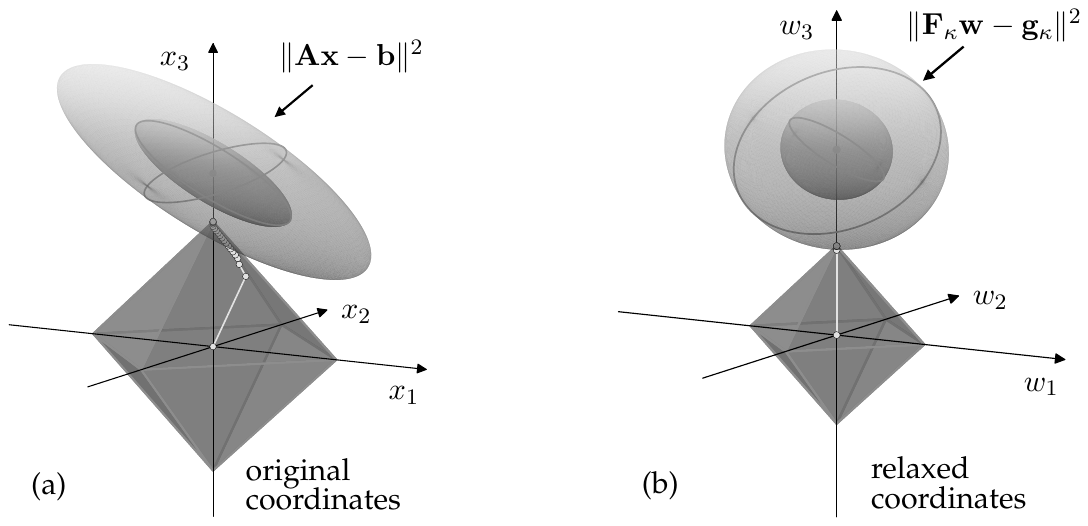
\includegraphics[width=.56\textwidth]{images/fig_5_3.png}
  \end{center}
  \vspace{-2mm}
  {\scriptsize\color{gray}
   Fig.~5.3 (p.~177): (a) conjuntos de nivel (elipses verdes) de la parte
   cuadrática de LASSO y el camino del gradiente proximal (40 iteraciones) en
   coordenadas $x$. (b) conjuntos de nivel (esferas verdes) de la pérdida SR3
   y el camino SR3 (2 iteraciones) en coordenadas relajadas $w$.}
  \begin{itemize}
    \item Minimizar parcialmente en $x$ deja una función enteramente en $z$ con
      conjuntos de nivel \textbf{casi esféricos}, frente a las elipses
      muy excéntricas de $\norm{Ax-b}_2^2$.
    \item SR3 disminuye los valores singulares de $F_\kappa$ respecto de $A$
      con menos efecto en los pequeños: ``aplasta'' las elipses en esferas
      $\to$ convergencia más rápida.
  \end{itemize}
  \fuente
\end{frame}

\begin{frame}{R5.15 --- Falsos positivos: LASSO frente a SR3}
  \small
  \begin{center}
    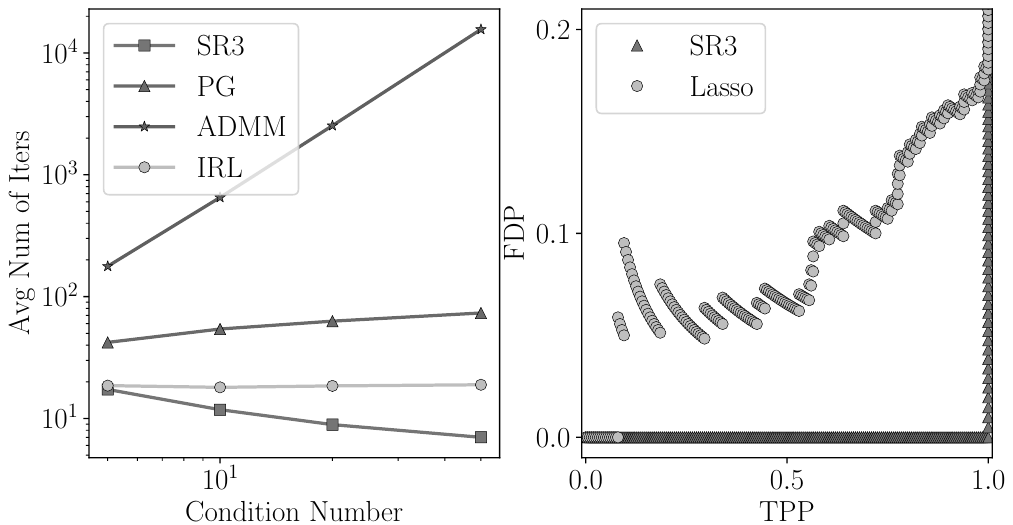
\includegraphics[width=.52\textwidth]{images/fig_5_4.png}
  \end{center}
  \vspace{-2mm}
  {\scriptsize\color{gray}
   Fig.~5.4 (p.~177): (izq. arriba) SR3 (rojo) es órdenes de magnitud más
   rápido que ADMM (verde) o el gradiente proximal (gris); IRL (azul) requiere
   iteraciones comparables pero con costo por iteración mayor.
   (der. arriba) verdaderos vs.~falsos positivos a lo largo del camino.}
  \begin{itemize}
    \item En LASSO los falsos positivos aparecen \textbf{temprano} en el camino
      de optimización y \textbf{no se pueden revertir}.
    \item Se atribuye a la excentricidad de la geometría del problema, que
      SR3 mitiga en gran medida: en SR3 casi no hay falsos positivos.
  \end{itemize}
  \fuente
\end{frame}

% =============================================================================
\section{Búsqueda sin derivadas}
% =============================================================================

\begin{frame}{Nelder--Mead: el marco}
  \small
  \begin{columns}[T,onlytextwidth]
    \begin{column}{.48\textwidth}
      \begin{itemize}
        \item \textbf{Nelder \& Mead, 1965}: búsqueda local sin gradiente para
          problemas sin restricciones.
        \item Trabaja \textbf{solo con evaluaciones de la función}: útil si el
          objetivo no es diferenciable, o si el gradiente numérico es caro o
          ruidoso.
        \item Funciona bien en \textbf{dimensiones bajas} (unas decenas de
          variables).
      \end{itemize}
    \end{column}
    \begin{column}{.48\textwidth}
      \begin{block}{Advertencia del libro (p.~178)}
        \small
        \emph{``A pesar de su popularidad... el método de Nelder--Mead \textbf{no
        tiene fuertes garantías teóricas de convergencia}. De hecho, hay
        contraejemplos conocidos, incluso para funciones estrictamente
        convexas, donde el método falla en converger o su desempeño se
        degrada.''}
      \end{block}
      \vspace{1mm}
      {\footnotesize\color{gray}
       \textbf{No confundir} con el método simplex de Dantzig del Cap.~3
       (programación lineal).}
    \end{column}
  \end{columns}
\end{frame}

\begin{frame}{R5.16--R5.17 --- La idea del simplex}
  \small
  \begin{itemize}
    \item Se inicializa un \textbf{simplex} en $\R^n$ con $n+1$ vértices
      $\{x_j\}$ y se evalúa $f$ en todos ellos.
    \item Se modifica el vértice con el \textbf{mayor} valor de $f$ para
      moverlo hacia un valor menor: el simplex ``rueda colina abajo''.
    \item Se asume el orden $f(x_0) \le f(x_1) \le \cdots \le f(x_n)$, y se
      define el \textbf{centroide de los $n$ mejores puntos}:
      \[
        \bar{x} = \frac{1}{n}\sum_{j=0}^{n-1} x_j
      \]
  \end{itemize}
  \vspace{-3mm}
  \begin{center}
    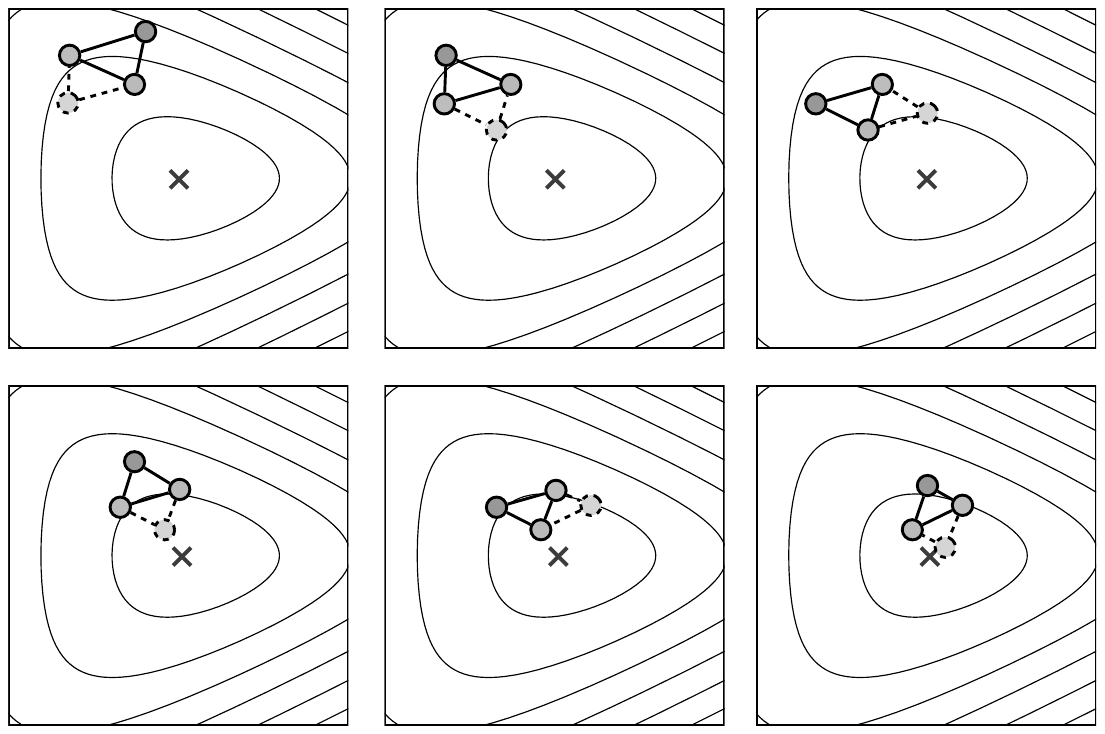
\includegraphics[width=.30\textwidth]{images/fig_5_5.png}
  \end{center}
  \vspace{-5mm}
  {\scriptsize\color{gray}
   Fig.~5.5 (p.~179): esquema del downhill simplex. El vértice rojo (peor valor)
   se refleja al vértice gris discontinuo; aquí las reflexiones simples bastan.}
  \fuente
\end{frame}

\begin{frame}{R5.18 --- Las cuatro operaciones}
  \small
  \begin{columns}[T,onlytextwidth]
    \begin{column}{.50\textwidth}
      \begin{enumerate}
        \item \textbf{Reflexión:} $x' = \bar{x}+\alpha(\bar{x}-x_n)$, con
          $\alpha\approx1$. Si $f(x_0)\le f(x')<f(x_{n-1})$, se acepta $x'$ y
          se reinicia el ciclo.
        \item \textbf{Expansión:} si $f(x')<f(x_0)$,
          $x'' = \bar{x}+\gamma(\bar{x}-x_n)$, con $\gamma\approx2\alpha>1$.
        \item \textbf{Contracción:} si $f(x')\ge f(x_{n-1})$,
          $x'' = \bar{x}+\rho(\bar{x}-x_n)$, con $\rho\approx0.5\alpha<1$.
        \item \textbf{Shrink:} si todo falla, ``como un balde de agua fría'':
          $x_i \leftarrow x_0+\sigma(x_i-x_0)$, con $0<\sigma<1$.
      \end{enumerate}
      \vspace{1mm}
      {\footnotesize\color{gray}
       Cada paso empieza en reflexión; el ranking de $f(x')$ decide si se
       acepta, se expande o se contrae. Sólo si todo falla se hace
       \emph{shrink}, que contrae todos los vértices hacia el mejor $x_0$.}
    \end{column}
    \begin{column}{.46\textwidth}
      \begin{figure}
        \centering
        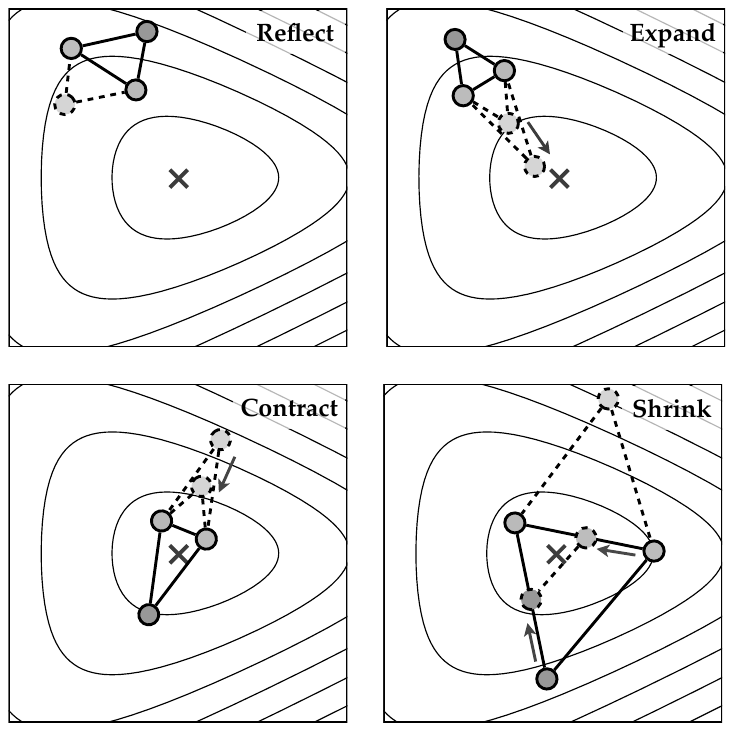
\includegraphics[width=.58\linewidth]{images/fig_5_6.png}
      \end{figure}
      \vspace{-2mm}
      {\scriptsize\color{gray}
       Fig.~5.6 (p.~181): las varias operaciones del downhill simplex.}
      \vspace{1mm}
      {\small\textbf{R5.19 --- Terminación}: valores de $f$ cercanos
      ($\max_j|f(x_j)-f(x_0)|<\epsilon$); tamaño del simplex bajo tolerancia;
      tope de evaluaciones o iteraciones.}
    \end{column}
  \end{columns}
  \fuente
\end{frame}

\begin{frame}{E5.3 --- El objetivo de prueba (Ec.~5.10)}
  \small
  \begin{columns}[T,onlytextwidth]
    \begin{column}{.54\textwidth}
      \[
        f(x) = 1 + \sum_{j=1}^{4} f_j(x), \qquad
        f_j(x) = -\alpha_j\, e^{-\frac{1}{2}\norm{x-x_j}_2^2}
      \]
      \[
        (\alpha_1,\dots,\alpha_4) = (3,\,1.5,\,1,\,2)
      \]
      \[
        x_1{=}(2,2),\; x_2{=}(-2,2),\; x_3{=}(2,-2),\; x_4{=}(-2,-2)
      \]
      \begin{itemize}
        \item Cuatro mínimos locales de profundidades distintas: el más
          profundo (profundidad $3$) está en $(2,2)$.
        \item El simplex parte de un simplex \emph{grande} en la esquina
          opuesta, así que debe escapar de los demás.
      \end{itemize}
    \end{column}
    \begin{column}{.42\textwidth}
      \begin{figure}
        \centering
        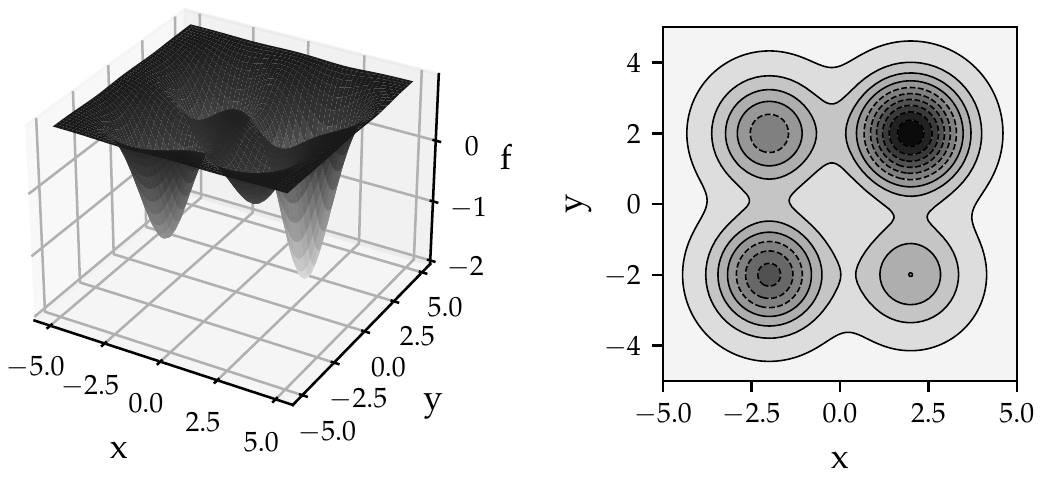
\includegraphics[width=\textwidth]{images/fig_5_7.png}
      \end{figure}
      \vspace{-2mm}
      {\scriptsize\color{gray}
       Fig.~5.7 (p.~182): el objetivo con cuatro mínimos locales, en 3D y en
       contornos.}
    \end{column}
  \end{columns}
  \fuente
\end{frame}

\begin{frame}[fragile]{E5.3 --- El downhill simplex en código}
  \small
  \begin{columns}[T,onlytextwidth]
    \begin{column}{.66\textwidth}
      \begin{lstlisting}[style=pythontiny]
def nelder_mead_step(vertices, alpha, gamma, rho, sigma):
    vals = np.array([f(v) for v in vertices])
    order = np.argsort(vals)
    vertices = vertices[order]; vals = vals[order]
    x1, x2, x3 = vertices   # best, middle, worst
    center = (x1 + x2) / 2.0
    x_reflect = center + alpha * (center - x3)   # Reflection
    f_reflect = f(x_reflect)
    if f_reflect < f1:         # Expansion
        x_expand = center + gamma * (x_reflect - center)
        vertices[2] = (x_expand if f(x_expand) < f_reflect
                       else x_reflect)
    elif f_reflect < f2:
        vertices[2] = x_reflect
    else:                      # worse than mid
        if f_reflect < f3:     # Outside contraction
            x_contr = center + rho * (x_reflect - center)
            if f(x_contr) <= f_reflect:
                vertices[2] = x_contr
            else:              # Shrink
                vertices[1] = x1 + sigma*(x2 - x1)
                vertices[2] = x1 + sigma*(x3 - x1)
        else:                  # Inside contraction
            x_contr = center - rho * (center - x3)
            if f(x_contr) < f3:
                vertices[2] = x_contr
            else:              # Shrink
                vertices[1] = x1 + sigma*(x2 - x1)
                vertices[2] = x1 + sigma*(x3 - x1)
    return vertices
      \end{lstlisting}
    \end{column}
    \begin{column}{.30\textwidth}
      \begin{lstlisting}[style=pythontiny]
vertices = np.array([[4.0, 4.0],
    [-4.0, -3.0],
    [-2.0, 4.0]])
for it in range(1, 31):
    vertices = nelder_mead_step(vertices)
      \end{lstlisting}
      \vspace{1mm}
      {\footnotesize\color{gray}
       El código ordena los vértices por valor, refleja el peor, y decide
       expand / accept / contract / shrink según el ranking del punto
       reflejado.}
    \end{column}
  \end{columns}
  \fuente
\end{frame}

\begin{frame}{E5.3 --- Resultado: el simplex encuentra el mínimo global}
  \small
  \begin{columns}[T,onlytextwidth]
    \begin{column}{.46\textwidth}
      \begin{figure}
        \centering
        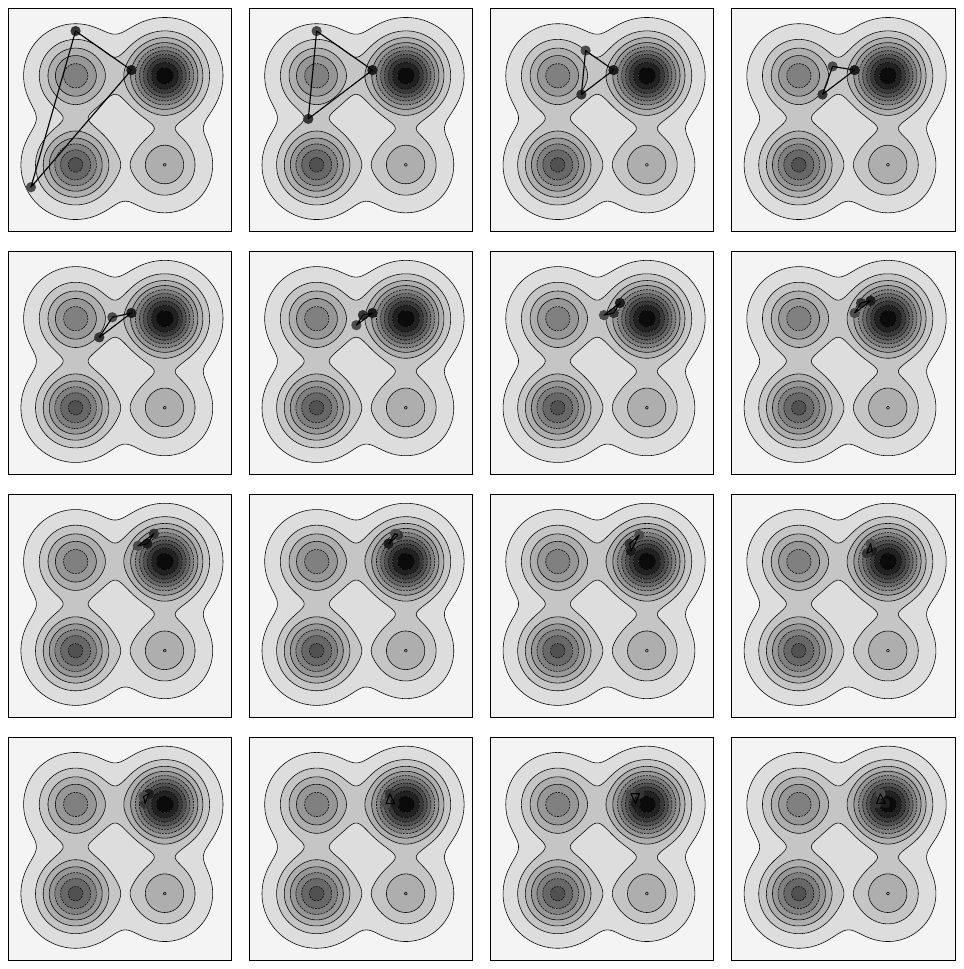
\includegraphics[width=.82\textwidth]{images/fig_5_9.png}
      \end{figure}
      \vspace{-1mm}
      {\scriptsize\color{gray}
       Fig.~5.9 (p.~184): la evolución del simplex. Tras una fase de
       exploración, encuentra el mínimo global.}
    \end{column}
    \begin{column}{.50\textwidth}
      \begin{figure}
        \centering
        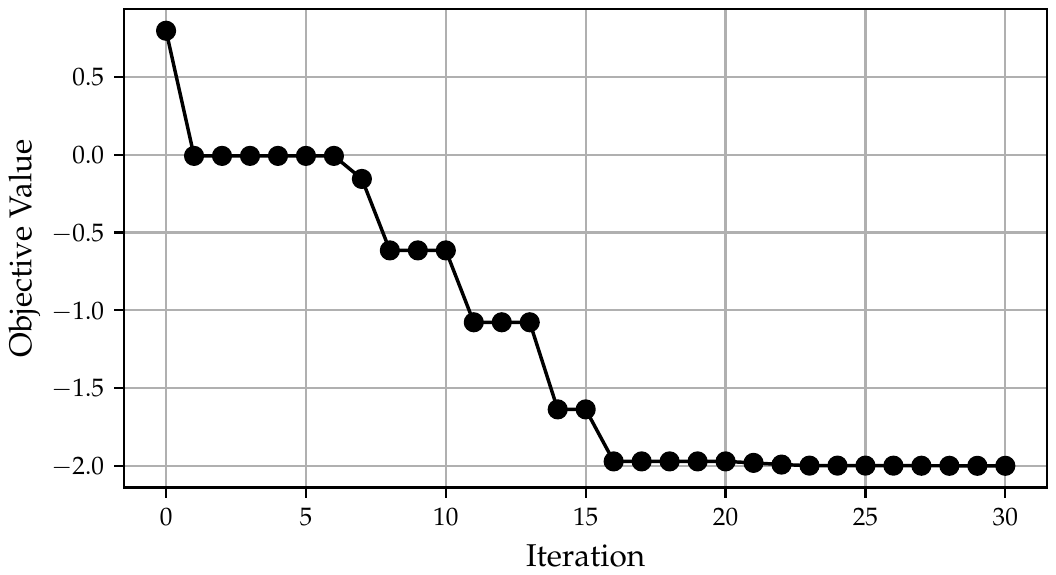
\includegraphics[width=.80\linewidth]{images/fig_5_8.png}
      \end{figure}
      \vspace{-2mm}
      {\scriptsize\color{gray}
       Fig.~5.8 (p.~183): la función objetivo contra iteración.}
      \vspace{1mm}
      {\footnotesize\color{gray}
       \emph{``Tras una búsqueda inicial, encuentra el mínimo global y entonces
       desciende al mejor valor.''} (p.~183)}
    \end{column}
  \end{columns}
  \fuente
\end{frame}

\begin{frame}{E5.3 --- Fortalezas, debilidades y veredicto}
  \small
  \begin{columns}[T,onlytextwidth]
    \begin{column}{.48\textwidth}
      \begin{block}{Fortalezas}
        \small
        Simple de implementar; no requiere gradiente ni derivadas de orden
        superior; bueno a pequeña escala cuando las evaluaciones de función
        son caras.
      \end{block}
      \begin{block}{Debilidades}
        \small
        Pocas garantías de convergencia; \textbf{converger a un mínimo local no
        garantiza que sea global}; mal rendimiento en dimensiones altas;
        puede estancarse sin un ajuste cuidadoso.
      \end{block}
    \end{column}
    \begin{column}{.48\textwidth}
      \begin{block}{Veredicto del libro (p.~180)}
        \small
        El downhill simplex de Nelder--Mead sigue siendo una de las técnicas
        de optimización local \emph{sin derivadas} más ampliamente usadas.
      \end{block}
      \begin{itemize}
        \item Su marco conceptual simple y el ajuste relativamente directo de
          sus hiperparámetros lo hacen atractivo en \textbf{dimensiones bajas a
          moderadas}.
        \item Especialmente cuando las evaluaciones de función son caras o
          ruidosas, pero se prefiere un método local para refinar cerca de un
          óptimo sospechado.
      \end{itemize}
    \end{column}
  \end{columns}
  \fuente
\end{frame}

\begin{frame}{Recocido simulado: la metáfora del temple}
  \small
  \begin{columns}[T,onlytextwidth]
    \begin{column}{.48\textwidth}
      \begin{itemize}
        \item Inspirado en el \textbf{temple metalúrgico}: calentar y enfriar
          lentamente para disminuir defectos y obtener una estructura
          cristalina fuerte.
        \item La \textbf{temperatura} es el \emph{tamaño de paso} de las
          perturbaciones aleatorias: temperatura alta $\Rightarrow$
          fluctuaciones grandes y exploratorias.
        \item No requiere gradiente; maneja objetivos estocásticos o ruidosos,
          y variables discretas, continuas o mixtas.
        \item Simple de implementar: sólo evaluaciones de $f$ y lógica básica.
      \end{itemize}
    \end{column}
    \begin{column}{.48\textwidth}
      \begin{figure}
        \centering
        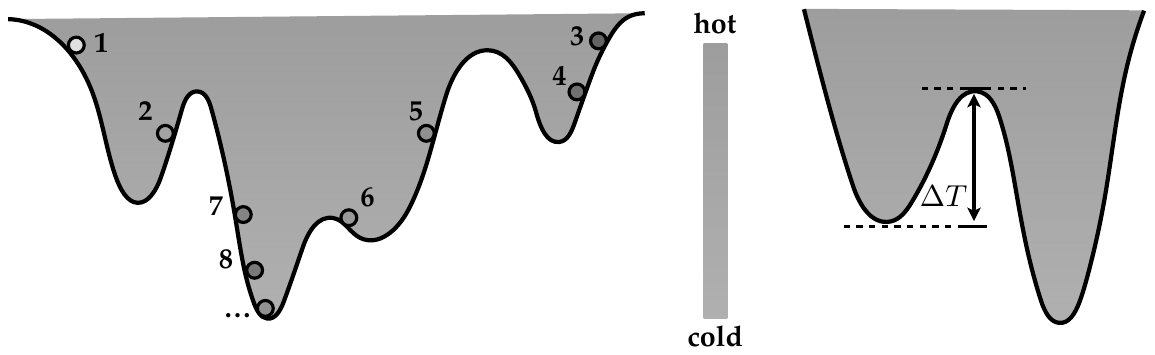
\includegraphics[width=\textwidth]{images/fig_5_10.png}
      \end{figure}
      \vspace{-1mm}
      {\scriptsize\color{gray}
       Fig.~5.10 (p.~186): esquema del recocido simulado. El camino de la
       variable de decisión pasa de ``caliente'' (amarillo/rojo) a ``frío''
       (azul); la temperatura determina la probabilidad de saltar de un
       mínimo local a otro.}
      \vspace{1mm}
      {\footnotesize\color{gray}
       Sobre la teoría (p.~186): hay resultados de convergencia en el límite
       de tiempo infinito, pero \textbf{no hay garantía de encontrar un mínimo
       global en tiempo finito}.}
    \end{column}
  \end{columns}
\end{frame}

\begin{frame}{R5.20--R5.22 --- Aceptación, enfriamiento e hiperparámetros}
  \small
  \begin{columns}[T,onlytextwidth]
    \begin{column}{.48\textwidth}
      \begin{block}{R5.20 --- El algoritmo de aceptación (p.~186)}
        \small
        Se propone $x_{k+1}$ en el vecindario de $x_k$, y
        $\Delta = f(x_{k+1})-f(x_k)$:
        \begin{enumerate}
          \item $\Delta \le 0$: se acepta \textbf{incondicionalmente}.
          \item $\Delta > 0$: se acepta con probabilidad
            \[
              p = \exp\!\left(-\tfrac{\Delta}{T}\right)
            \]
        \end{enumerate}
      \end{block}
      \begin{block}{R5.21 --- Calendarios de enfriamiento}
        \small
        \[
          T_{k+1} = \alpha\, T_k,\qquad 0<\alpha<1
        \]
        \vspace{-2mm}
        {\scriptsize (p.~ej. $0.9 \le \alpha \le 0.99$)}
        Hay garantías teóricas para $T_k$ entre las curvas $1/k$ y $1/k^2$.
      \end{block}
    \end{column}
    \begin{column}{.48\textwidth}
      \textbf{R5.22 --- Hiperparámetros a ajustar (p.~187)}
      \begin{itemize}
        \item \textbf{Temperatura inicial $T_0$}: alta para aceptar
          movimientos peores al inicio y explorar globalmente. Si es demasiado
          grande, se necesitan muchas iteraciones antes de poder explotar
          localmente.
        \item \textbf{Factor de enfriamiento $\alpha$}: demasiado rápido y no
          hay tiempo de explorar; demasiado lento y no converge a un buen
          mínimo.
        \item \textbf{Operador de movimiento}: perturbaciones gaussianas o
          uniformes en dominios continuos; permutaciones aleatorias en
          discretos (e.g.~traveling salesman).
        \item \textbf{Criterios de terminación}: $T_{\min}$, tope de
          iteraciones, o estasis por $n$ pasos.
      \end{itemize}
    \end{column}
  \end{columns}
  \fuente
\end{frame}

\begin{frame}[fragile]{E5.4 --- El recocido simulado en código}
  \small
  \begin{columns}[T,onlytextwidth]
    \begin{column}{.56\textwidth}
      \begin{lstlisting}[style=pythontiny]
def simulated_annealing(init_point, n_iter=200, T0=5.0,
    alpha=0.98, step_size=1.0, bounds=(-5,5)):
    current = np.array(init_point, dtype=float)
    current_val = f(current)
    path = [current.copy()]
    temp = T0
    for i in range(n_iter):
        # Propose random step
        candidate = current + np.random.randn(2) * step_size
        candidate = np.clip(candidate, bounds[0], bounds[1])
        candidate_val = f(candidate)
        delta = candidate_val - current_val
        # Accept if better, or with prob. exp(-delta/T)
        if delta < 0:
            current, current_val = candidate, candidate_val
        else:
            if np.random.rand() < np.exp(-delta / temp):
                current, current_val = candidate, candidate_val
        temp *= alpha            # Lower the temperature
        path.append(current.copy())
    return np.array(path)

path = simulated_annealing(init_point=[-4.0,-4.0],
    n_iter=200, T0=10.0, alpha=0.98, step_size=1.)
      \end{lstlisting}
      \vspace{1mm}
      {\footnotesize\color{gray}
       Con \texttt{scipy}: \texttt{dual\_annealing(objective\_2d,
       bounds=[(-5,5),(-5,5)], maxiter=1000, seed=0)}; devuelve \texttt{x},
       \texttt{fun}, \texttt{nfev}, \texttt{nit}.}
    \end{column}
    \begin{column}{.40\textwidth}
      \begin{figure}
        \centering
        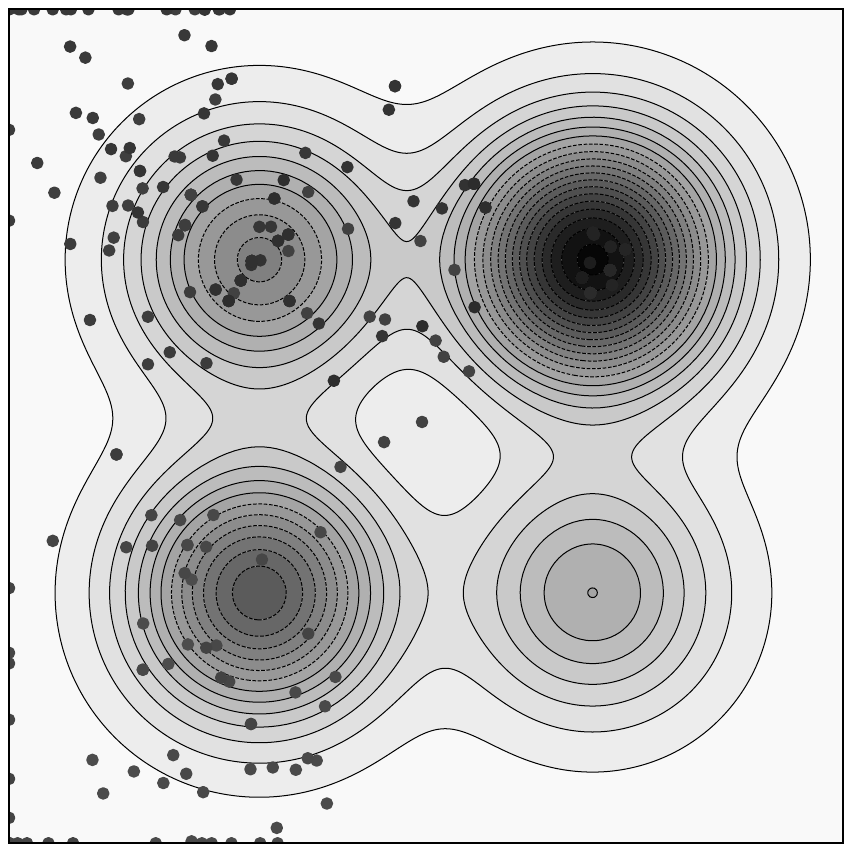
\includegraphics[width=.78\textwidth]{images/fig_5_11.png}
      \end{figure}
      \vspace{-2mm}
      {\scriptsize\color{gray}
       Fig.~5.11 (p.~188): los puntos ``calientes'' son rojos y se van
       enfriando hasta el azul. Eventualmente se encuentra el mínimo global.}
    \end{column}
  \end{columns}
  \fuente
\end{frame}

\begin{frame}{E5.4 --- Resultado: el ensemble de caminos}
  \small
  \begin{columns}[T,onlytextwidth]
    \begin{column}{.48\textwidth}
      \begin{figure}
        \centering
        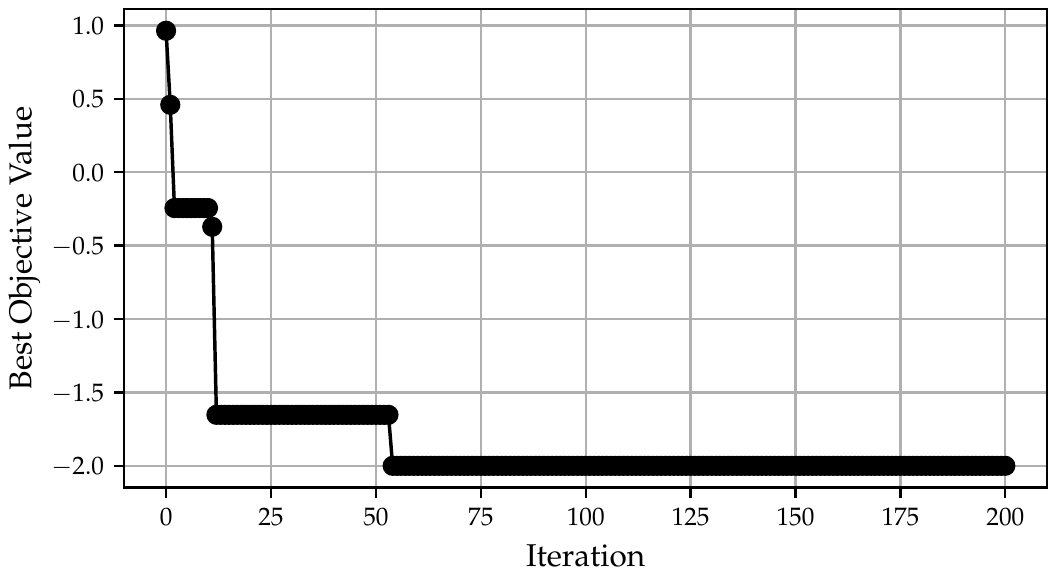
\includegraphics[width=\textwidth]{images/fig_5_12.png}
      \end{figure}
      \vspace{-2mm}
      {\scriptsize\color{gray}
       Fig.~5.12 (p.~189): la función objetivo contra iteración.}
    \end{column}
    \begin{column}{.48\textwidth}
      \begin{figure}
        \centering
        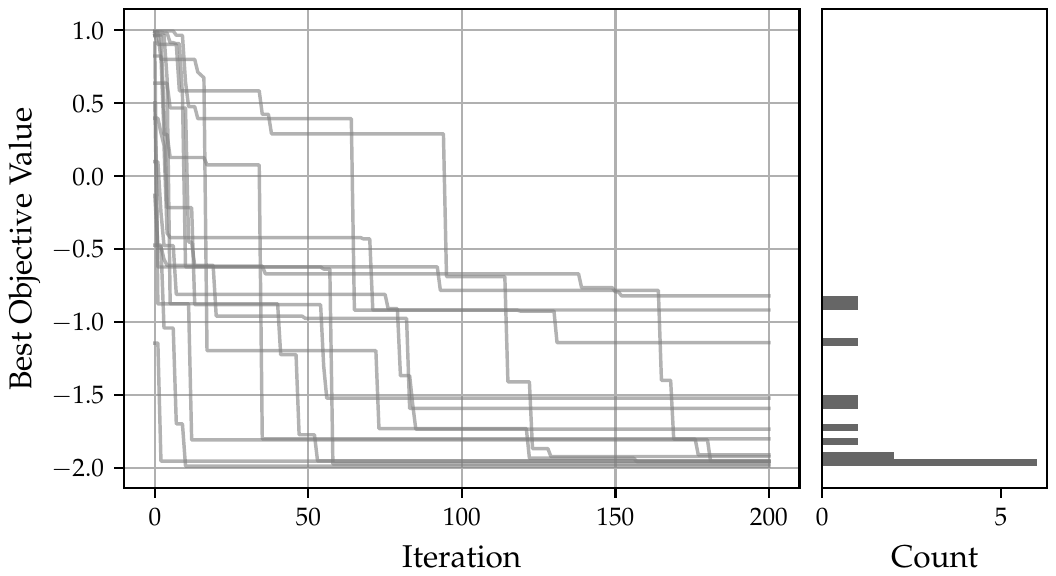
\includegraphics[width=\textwidth]{images/fig_5_13.png}
      \end{figure}
      \vspace{-2mm}
      {\scriptsize\color{gray}
       Fig.~5.13 (p.~189): conjunto (ensemble) de múltiples caminos de recocido
       simulado, con un histograma del valor optimizado final.}
    \end{column}
  \end{columns}
  \vspace{1mm}
  {\footnotesize\color{gray}
   \emph{``Es ilustrativo repetir este proceso para un \emph{ensemble} de muchos
   caminos de temple, para ver cómo evoluciona la distribución con el número
   de iteración.''} (p.~189)}
  \fuente
\end{frame}

% =============================================================================
\section{Algoritmos evolutivos}
% =============================================================================

\begin{frame}{Algoritmos evolutivos: el marco}
  \small
  \begin{columns}[T,onlytextwidth]
    \begin{column}{.48\textwidth}
      \begin{itemize}
        \item Basados en evolución biológica y supervivencia del más apto:
          \textbf{replicación, mutación e intercambio de información genética}.
        \item Se evoluciona iterativamente una \textbf{población} de soluciones
          candidatas; con buenos hiperparámetros la distribución de desempeño
          mejora y los individuos se acercan al óptimo global.
      \end{itemize}
      \begin{block}{Las dos categorías}
        \small
        \textbf{Optimización de parámetros}: se aprende $\theta$ de una
        estructura conocida (ajustar $\hat y=f_\theta(x)$, o las ganancias de
        un controlador).
        \par\medskip
        \textbf{Optimización de funciones}: se aprende \emph{la estructura y los
        parámetros} a la vez.
      \end{block}
    \end{column}
    \begin{column}{.48\textwidth}
      \begin{figure}
        \centering
        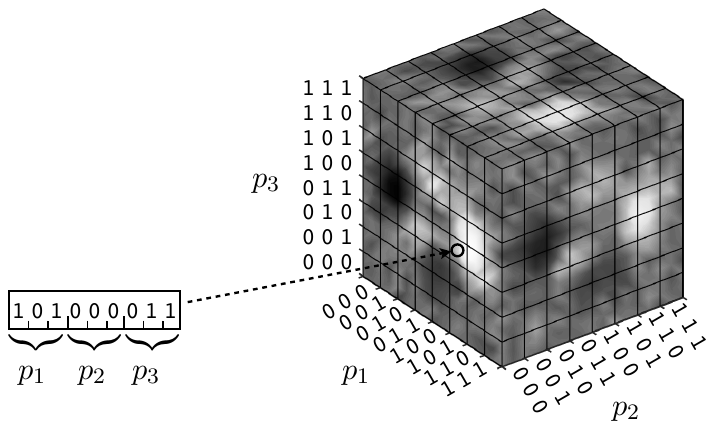
\includegraphics[width=\textwidth]{images/fig_5_14.png}
      \end{figure}
      \vspace{-1mm}
      {\scriptsize\color{gray}
       Fig.~5.14 (p.~191): cubo de parámetros $p_1,p_2,p_3$ (e.g.~gancias de un
       PID). El GA codifica un valor como secuencia binaria: \texttt{000} es el
       límite inferior, \texttt{111} el superior. El color es el costo.}
      \vspace{1mm}
      {\footnotesize\color{gray}
       La programación genética suele llamarse \textbf{regresión simbólica}: da
       representaciones analíticas de la función optimizada, útil para la
       \textbf{IA explicable}.}
    \end{column}
  \end{columns}
\end{frame}

\begin{frame}{R5.23 --- Las cuatro operaciones genéticas}
  \small
  \begin{columns}[T,onlytextwidth]
    \begin{column}{.54\textwidth}
      \begin{tabular}{@{}p{.26\textwidth}p{.66\textwidth}@{}}
        \toprule
        \textbf{Operación} & \textbf{Efecto (libro, p.~190)} \\
        \midrule
        Replication & Propaga el individuo seleccionado a la siguiente
          generación. \\
        Crossover & Dos individuos intercambian parte de su código: explota y
          mejora estrategias exitosas. \\
        Mutation & Se modifica parte del código con valores nuevos: promueve
          la diversidad y la exploración. \\
        Elitism & Un número fijo de los mejores avanza directo a la siguiente
          generación (opcional). \\
        \bottomrule
      \end{tabular}
      \vspace{2mm}
      \begin{itemize}
        \item Los individuos se seleccionan al azar con \textbf{probabilidad
          proporcional a la aptitud}.
        \item Se itera hasta que las estadísticas de la población convergen.
      \end{itemize}
    \end{column}
    \begin{column}{.42\textwidth}
      \begin{figure}
        \centering
        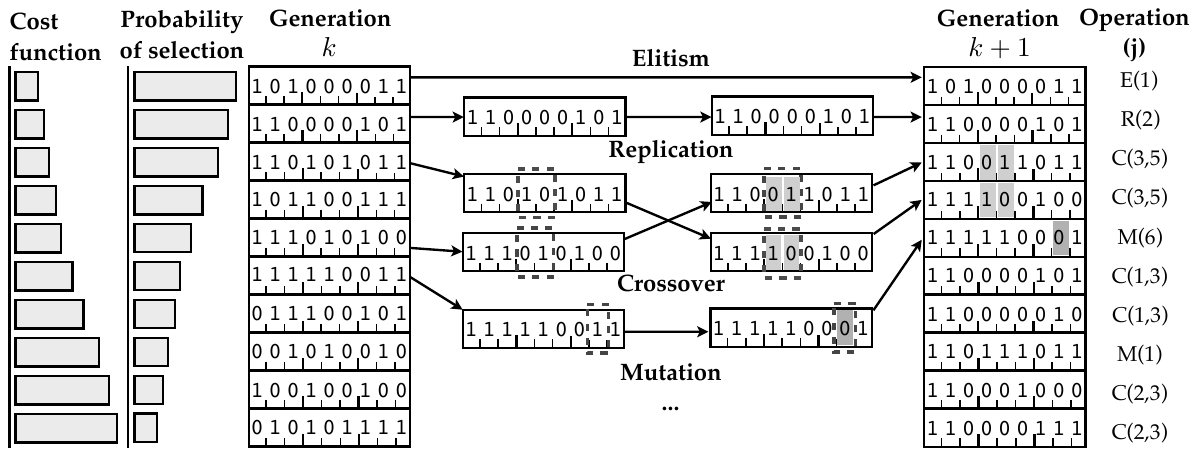
\includegraphics[width=\textwidth]{images/fig_5_15.png}
      \end{figure}
      \vspace{-1mm}
      {\scriptsize\color{gray}
       Fig.~5.15 (p.~191): los individuos de la generación $k$ se evalúan y
       clasifican; se eligen con probabilidad ponderada para la generación
       $k+1$ mediante elitismo, replicación, crossover y mutación.}
    \end{column}
  \end{columns}
  \fuente
\end{frame}

\begin{frame}{R5.24--R5.25 --- Garantías e hiperparámetros}
  \small
  \begin{columns}[T,onlytextwidth]
    \begin{column}{.48\textwidth}
      \begin{block}{R5.24 --- No hay garantía de óptimo global}
        \small
        Los GA encuentran valores \emph{casi} globalmente óptimos: exploran y
        explotan pozos locales. Son un \textbf{punto medio entre la fuerza
        bruta y la optimización convexa}, y una alternativa al muestreo Monte
        Carlo caro, que no escala a espacios de alta dimensión.
        \par\medskip
        \textbf{Pero no hay garantía de convergencia a un óptimo global.}
      \end{block}
      \textbf{R5.25 --- Hiperparámetros}:
      \begin{itemize}
        \item tamaño de las poblaciones;
        \item número de generaciones;
        \item tasas de selección relativas de cada operación.
      \end{itemize}
    \end{column}
    \begin{column}{.48\textwidth}
      \begin{block}{R5.26--R5.27 --- Programación genética}
        \small
        GP optimiza \textbf{simultáneamente estructura y parámetros} de un mapa
        entrada--salida.
        \par\medskip
        Representación en \textbf{árbol de funciones}: cada rama es una señal y
        los puntos de fusión son operaciones matemáticas; las entradas y
        constantes son las \textbf{hojas}, y la salida de $f(x)$ es la
        \textbf{raíz}. Las operaciones genéticas actúan sobre el árbol con
        probabilidades $p(C)$, $p(M)$ y $p(R)$.
      \end{block}
      \vspace{1mm}
      \begin{figure}
        \centering
        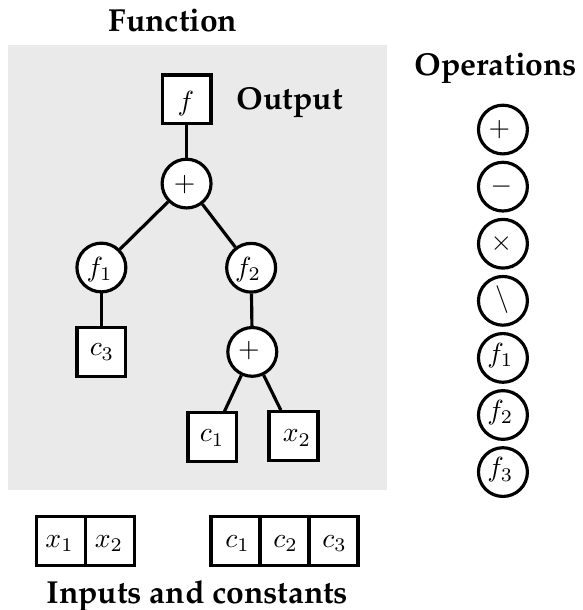
\includegraphics[width=.24\textwidth]{images/fig_5_16.png}
      \end{figure}
      \vspace{-2mm}
      {\scriptsize\color{gray}
       Fig.~5.16 (p.~192): el árbol de funciones que representa $f(x)$.}
    \end{column}
  \end{columns}
  \fuente
\end{frame}

\begin{frame}[fragile]{E5.5 --- Regresión simbólica con PySR}
  \small
  \begin{columns}[T,onlytextwidth]
    \begin{column}{.55\textwidth}
      \begin{lstlisting}[style=pythontiny]
from pysr import PySRRegressor
from sympy import lambdify, symbols

# Generate data from Lorenz system
x0 = [5, 5, 5]
sol_train = solve_ivp(lorenz, (0, 2), x0, t_eval=t_train)
X_train = sol_train.y.T
dXdt_train = np.gradient(X_train, dt, axis=0)

# Train PySR models for dx/dt, dy/dt, dz/dt
variables = symbols("x0 x1 x2")
for i, label in enumerate(["dx/dt","dy/dt","dz/dt"]):
    model = PySRRegressor(
        model_selection="best",
        binary_operators=["+","-","*","/"],
        unary_operators=["sin","cos","exp"],
        loss="loss(x, y) = (x - y)^2",
        niterations=100, maxsize=10, populations=10)
    model.fit(X_train, dXdt_train[:, i])
      \end{lstlisting}
    \end{column}
    \begin{column}{.41\textwidth}
      \begin{itemize}
        \item Se generan datos del sistema de Lorenz y se calculan las
          derivadas \emph{por diferencias finitas}.
        \item Un modelo por cada componente: se aprende la \emph{estructura}
          y los parámetros a la vez.
        \item El libro anticipa: esto se revisita como problema inverso en el
          Cap.~8.
      \end{itemize}
      \begin{block}{R5.28 --- Pocas garantías teóricas}
        \small
        Aunque los algoritmos evolutivos son extremadamente generales y
        poderosos, hay muy pocas garantías teóricas de convergencia y
        estabilidad.
      \end{block}
    \end{column}
  \end{columns}
  \fuente
\end{frame}

\begin{frame}{E5.5 --- Resultado: el sistema de Lorenz aprendido}
  \small
  \begin{columns}[T,onlytextwidth]
    \begin{column}{.54\textwidth}
      \begin{figure}
        \centering
        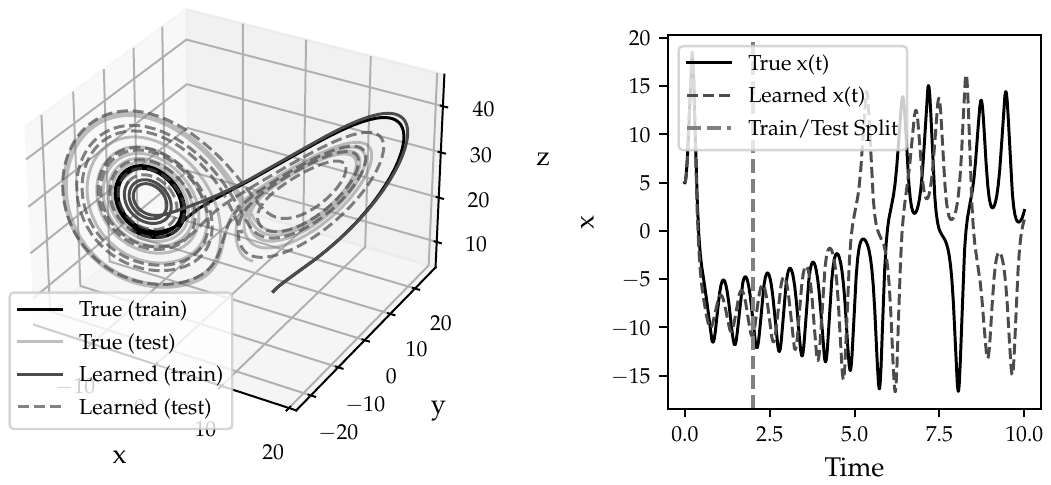
\includegraphics[width=\textwidth]{images/fig_5_18.png}
      \end{figure}
      \vspace{-2mm}
      {\scriptsize\color{gray}
       Fig.~5.18 (p.~194): salida de PySR sobre el sistema de Lorenz. El modelo
       se entrena en las primeras 2 unidades de tiempo y se prueba en las
       siguientes 8; el desempeño está en excelente acuerdo.}
    \end{column}
    \begin{column}{.42\textwidth}
      \begin{figure}
        \centering
        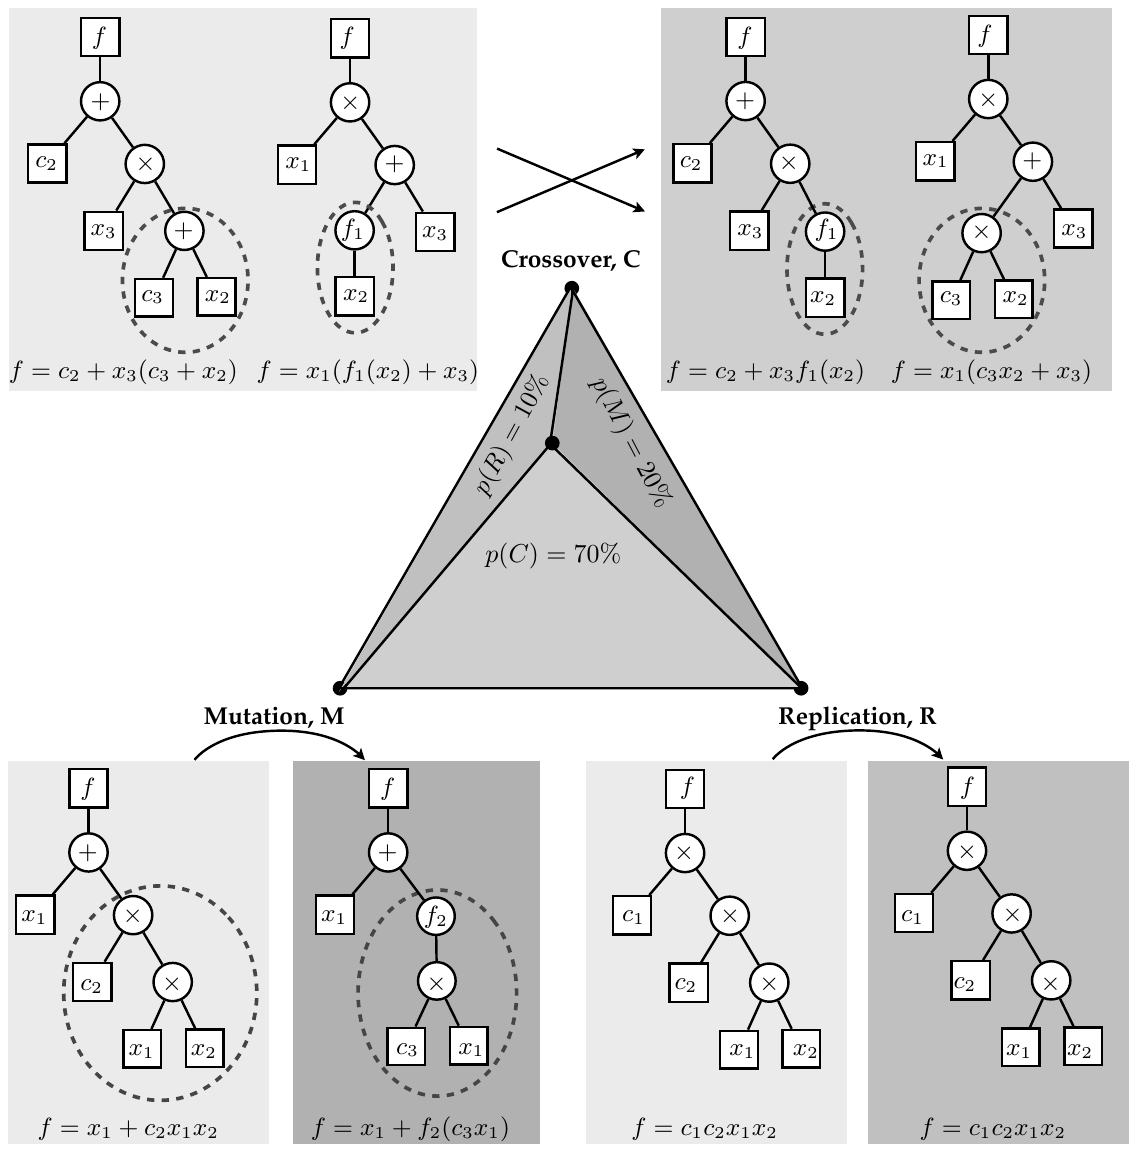
\includegraphics[width=.55\linewidth]{images/fig_5_17.png}
      \end{figure}
      \vspace{-2mm}
      {\scriptsize\color{gray}
       Fig.~5.17 (p.~193): operaciones genéticas sobre los árboles de funciones.
       En el ejemplo, $p(R)=10\%$, $p(M)=20\%$ y $p(C)=70\%$.}
      \vspace{2mm}
      {\footnotesize\color{gray}
       \textbf{IA explicable}: la regresión simbólica devuelve una fórmula
       legible, no una caja negra.}
    \end{column}
  \end{columns}
  \fuente
\end{frame}

\begin{frame}{Dos paradigmas para problemas grandes}
  \small
  \begin{columns}[T,onlytextwidth]
    \begin{column}{.48\textwidth}
      \begin{block}{Optimización distribuida}
        \small
        Descompone el problema en subproblemas que corren en \textbf{paralelo},
        sincronizando soluciones parciales por protocolos de comunicación.
        \par\medskip
        \textbf{Ventajas}: escalabilidad, privacidad (los datos pueden quedar
        locales en cada nodo --- p.ej.~aprendizaje federado), paralelismo
        eficiente.
        \par\medskip
        \textbf{Desventajas}: complejidad de implementación (asincronía,
        paso de mensajes), convergencia más lenta que la de un solucionador
        centralizado, y dependencia de la fiabilidad de la comunicación y de la
        topología de la red.
      \end{block}
    \end{column}
    \begin{column}{.48\textwidth}
      \begin{block}{Optimización por enjambre}
        \small
        Se inspira en bandadas de aves, cardúmenes de peces y hormigas
        forrajeando: la \textbf{calidad global emerge} de cómo interactúan
        muchos agentes simples y se autoactualizan.
        \par\medskip
        \textbf{Ventajas}: fácil de implementar, versátil para problemas de caja
        negra o no suaves, paralelizable.
        \par\medskip
        \textbf{Limitaciones}: sin garantías exactas, sensible a los
        hiperparámetros, y el escalamiento no siempre es favorable.
      \end{block}
      \vspace{1mm}
      {\footnotesize\color{gray}
       Síntesis del libro (p.~195): ambos son \textbf{toma de decisiones
       colectiva}; la optimización distribuida se apoya en una descomposición
       matemática rigurosa, y los métodos de enjambre en procesos de búsqueda
       iterativos guiados por heurísticas y coordinación emergente.}
    \end{column}
  \end{columns}
\end{frame}

\begin{frame}{R5.29--R5.31 --- Optimización distribuida}
  \small
  \begin{columns}[T,onlytextwidth]
    \begin{column}{.48\textwidth}
      \textbf{R5.29 --- Formulación (p.~195)}
      \[
        \min_x f(x) = \sum_{j=1}^{m} f_j(x)
      \]
      \begin{itemize}
        \item Cada $f_j$ corresponde a un agente (o nodo) $j$ de la red; cada
          agente conoce \textbf{sólo su función local} $f_j$ y parte de los
          datos.
        \item Los agentes se comunican (gradientes, subgradientes o soluciones
          parciales) para encontrar colaborativamente un minimizador global
          $x^\ast$.
        \item El \textbf{consenso} es el concepto fundamental: todos acaban
          de acuerdo en un vector común.
      \end{itemize}
    \end{column}
    \begin{column}{.48\textwidth}
      \begin{block}{R5.30 --- ADMM como descomposición}
        \small
        El \textbf{método alterno de multiplicadores} descompone el problema
        grande en subproblemas, cada uno resuelto localmente, con actualizaciones
        que aseguran la consistencia global.
        \par\medskip
        El libro lo desarrolla en detalle en la \S6.5.
      \end{block}
      \vspace{1mm}
      {\footnotesize\color{gray}
       Antecedentes: control descentralizado y procesamiento paralelo en los
       años 1970--1980; luego redes de sensores, comunicaciones y aprendizaje
       federado. La \emph{swarm intelligence} tomó forma en los 90 con PSO
       (Kennedy y Eberhart) y ACO (Dorigo y coautores).}
    \end{column}
  \end{columns}
  \fuente
\end{frame}

\begin{frame}{R5.32--R5.33 --- Optimización por enjambre de partículas}
  \small
  \begin{columns}[T,onlytextwidth]
    \begin{column}{.52\textwidth}
      \begin{block}{Las ecuaciones de PSO (p.~196)}
        \small
        \[
          v_j^{(k+1)} = \omega v_j^{(k)}
          + c_1 r_1\big(x_j^{(k)*}-x_j^{(k)}\big)
          + c_2 r_2\big(x^{(k)*}-x_j^{(k)}\big)
        \]
        \[
          x_j^{(k+1)} = x_j^{(k)} + v_j^{(k+1)}
        \]
        \begin{itemize}
          \item $x_j^{(k)*}$: mejor posición histórica de la partícula $j$.
          \item $x^{(k)*}$: mejor global entre todas las partículas.
          \item $r_1,r_2 \in [0,1]$ aleatorios; $\omega, c_1, c_2$ balancean
            \textbf{exploración} y \textbf{explotación}.
        \end{itemize}
      \end{block}
    \end{column}
    \begin{column}{.44\textwidth}
      \begin{figure}
        \centering
        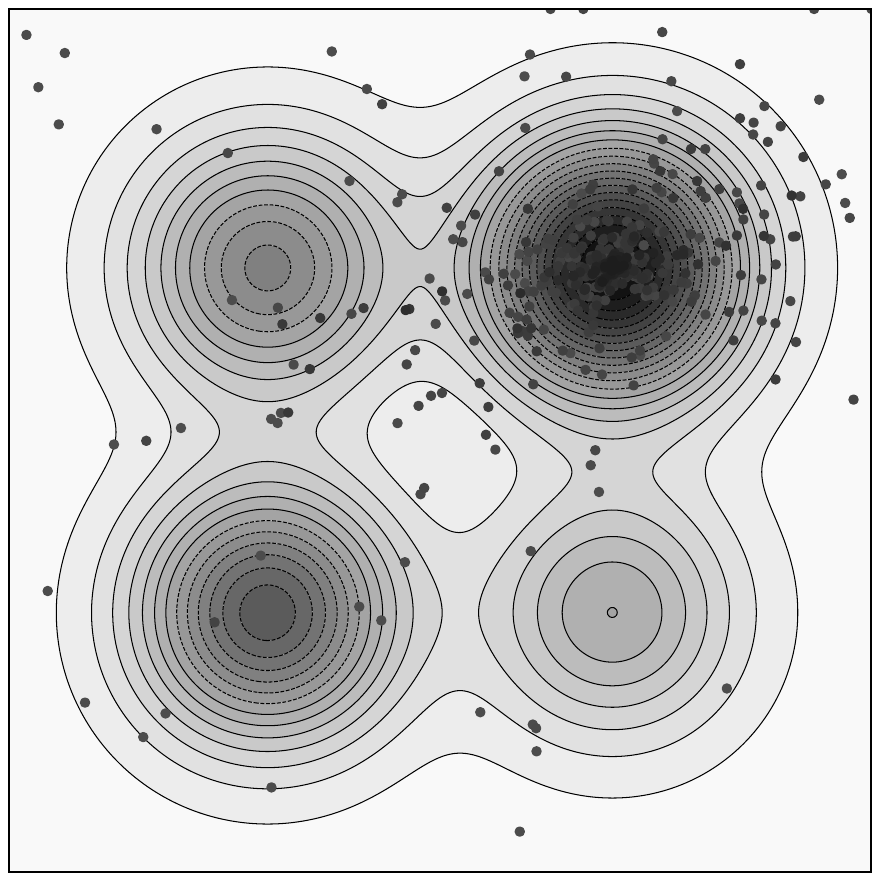
\includegraphics[width=.62\textwidth]{images/fig_5_19.png}
      \end{figure}
      \vspace{-2mm}
      {\scriptsize\color{gray}
       Fig.~5.19 (p.~197): las ubicaciones iniciales del enjambre en rojo se
       vuelven azules conforme optimizan. Eventualmente se encuentra el mínimo
       global.}
      \vspace{2mm}
      {\footnotesize\color{gray}
       El enjambre converge al óptimo en relativamente pocas iteraciones
       (Fig.~5.20).}
    \end{column}
  \end{columns}
  \fuente
\end{frame}

\begin{frame}[fragile]{E5.6 --- PSO en código}
  \small
  \begin{columns}[T,onlytextwidth]
    \begin{column}{.55\textwidth}
      \begin{lstlisting}[style=pythontiny]
def particle_swarm_optimization(n_particles=30, n_iter=20,
    w=0.5, c1=1.5, c2=1.5, bounds=(-5, 5)):
    positions = np.random.uniform(bounds[0], bounds[1],
        size=(n_particles, 2))
    velocities = np.zeros_like(positions)
    p_best = positions.copy()
    p_best_vals = np.apply_along_axis(
        lambda p: f(*p), 1, p_best)
    g_best = p_best[np.argmin(p_best_vals)]
    history = [positions.copy()]
    for _ in range(n_iter):
        r1 = np.random.rand(n_particles, 1)
        r2 = np.random.rand(n_particles, 1)
        velocities = (w * velocities
            + c1 * r1 * (p_best - positions)
            + c2 * r2 * (g_best - positions))
        positions = np.clip(positions + velocities,
            bounds[0], bounds[1])
        vals = np.apply_along_axis(
            lambda p: f(*p), 1, positions)
        improved = vals < p_best_vals
        p_best[improved] = positions[improved]
        p_best_vals[improved] = vals[improved]
    g_best = p_best[np.argmin(p_best_vals)]
    history.append(positions.copy())
    return np.array(history), g_best
      \end{lstlisting}
    \end{column}
    \begin{column}{.41\textwidth}
      \begin{itemize}
        \item Cada partícula guarda su \textbf{mejor posición personal}
          ($p\_best$) y el enjambre comparte el \textbf{mejor global}
          ($g\_best$).
        \item La velocidad mezcla tres términos: inercia ($\omega$),
          atracción personal ($c_1$) y atracción global ($c_2$).
        \item Las posiciones se recortan a la caja: el enjambre no puede
          salirse del dominio.
      \end{itemize}
    \end{column}
  \end{columns}
  \fuente
\end{frame}

\begin{frame}{E5.6 --- Resultado: convergencia del enjambre}
  \small
  \begin{columns}[T,onlytextwidth]
    \begin{column}{.46\textwidth}
      \begin{figure}
        \centering
        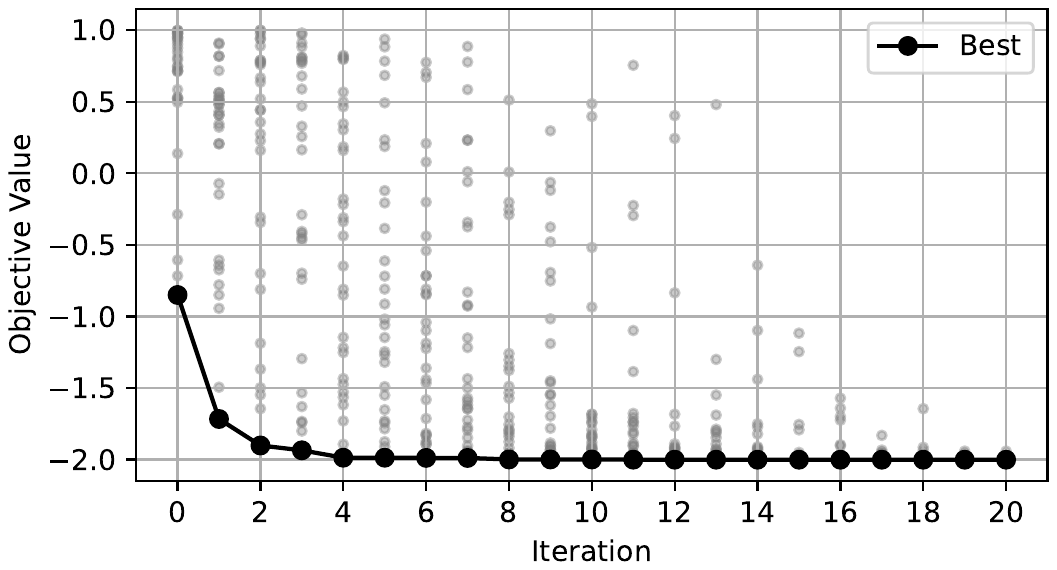
\includegraphics[width=\textwidth]{images/fig_5_20.png}
      \end{figure}
      \vspace{-2mm}
      {\scriptsize\color{gray}
       Fig.~5.20 (p.~198): la función objetivo contra iteración para PSO.}
    \end{column}
    \begin{column}{.50\textwidth}
      \begin{block}{R5.36 --- Convergencia colectiva}
        \small
        PSO y ACO se apoyan en reglas locales simples a nivel de agente; aun
        así, el sistema colectivo converge a soluciones de alta calidad, incluso
        en paisajes complejos. Las pruebas dependen de supuestos sobre la
        estructura del problema y el ajuste de parámetros.
      \end{block}
      \vspace{1mm}
      {\footnotesize\color{gray}
       El enjambre converge al óptimo en relativamente pocas iteraciones: no
       hace falta conocer el gradiente, ni la curvatura, ni la estructura del
       problema.}
    \end{column}
  \end{columns}
  \fuente
\end{frame}

\begin{frame}{R5.34--R5.35 --- Optimización por colonia de hormigas}
  \small
  \begin{columns}[T,onlytextwidth]
    \begin{column}{.52\textwidth}
      \textbf{ACO (Dorigo y coautores)} representa las soluciones como
      \textbf{caminos en un grafo}. Cada hormiga elige su siguiente arista con
      probabilidad
      \[
        P_{i,j} = \frac{\tau_{i,j}^{\alpha}\ \eta_{i,j}^{\beta}}
        {\sum_{k \in N_i} \tau_{i,k}^{\alpha}\ \eta_{i,k}^{\beta}}
      \]
      \begin{itemize}
        \item $\tau_{i,j}$: \textbf{nivel de feromona} en la arista $(i,j)$.
        \item $\eta_{i,j}$: \textbf{medida heurística} (p.ej.~el inverso de la
          distancia).
        \item $\alpha,\beta$: peso relativo de la feromona frente a la
          heurística.
      \end{itemize}
    \end{column}
    \begin{column}{.44\textwidth}
      \begin{block}{Actualización de feromonas}
        \small
        \[
          \tau_{i,j} \leftarrow (1-\rho)\,\tau_{i,j}
          + \sum_{\text{hormigas }k} \Delta\tau_{i,j}^{k}
        \]
        \[
          \Delta\tau_{i,j}^{k} = \begin{cases}
            Q/L_k, & \text{si la hormiga } k \text{ usó } (i,j)\\
            0, & \text{en otro caso}
          \end{cases}
        \]
        Con tasa de evaporación $\rho\in(0,1]$: se refuerzan las aristas
        prometedoras y las demás se evaporan.
      \end{block}
    \end{column}
  \end{columns}
  \fuente
\end{frame}

% =============================================================================
\section{Cierre}
% =============================================================================

\begin{frame}{Puntos para recordar}
  \small
  \begin{enumerate}
    \item \textbf{El prox sustituye al gradiente:} define una operación que
      incorpora el término no suave; ya se conoce para decenas de
      regularizadores.
    \item \textbf{ISTA y hard thresholding:} el prox del $\ell_1$ es
      umbralización suave ($\tau=\lambda/\beta$); el del $\ell_0$ es
      umbralización dura ($\tau=\sqrt{2\lambda/\beta}$).
    \item \textbf{Proyección y separación:} el prox del indicador es la
      proyección; separar variables abre la puerta a SR3 y ADMM.
    \item \textbf{SR3 relaja y regulariza:} aplasta los conjuntos de nivel en
      esferas, converge en 2 iteraciones donde LASSO necesita 40, y elimina
      los falsos positivos del camino de LASSO.
    \item \textbf{Nelder--Mead, annealing, GA, PSO, ACO:} todos son
      heurísticas sin garantía de óptimo global; su valor está en la
      robustez y la facilidad de implementación.
    \item \textbf{El calendario de enfriamiento y la $T_0$} son las
      palancas que deciden si el recocido explota o converge.
  \end{enumerate}
  \fuente
\end{frame}

\begin{frame}{El mapa completo}
  \centering
  \small
  \vspace{2mm}
  \begin{tabular}{@{}p{0.32\textwidth}p{0.60\textwidth}@{}}
    \toprule
    \textbf{Herramienta} & \textbf{Qué problema resuelve} \\
    \midrule
    Gradiente proximal & $f$ suave $+ g$ no suave, sin fórmula cerrada \\
    Umbralización suave / dura & Prox del $\ell_1$ (ISTA) y del $\ell_0$ \\
    Gradiente proyectado & Restricciones de caja y conjuntos factibles \\
    Separación de variables & Problemas grandes o mal condicionados (SR3, ADMM) \\
    Nelder--Mead & Búsqueda local sin derivadas, dimensiones bajas \\
    Recocido simulado & Búsqueda global estocástica, objetivos ruidosos \\
    Algoritmos genéticos & Optimización de parámetros, espacios grandes \\
    Programación genética & Regresión simbólica, IA explicable \\
    PSO / ACO & Búsqueda por enjambre, problemas de caja negra \\
    \bottomrule
  \end{tabular}
  \vspace{4mm}
  {\footnotesize\color{gray}
    La pregunta de fondo del capítulo: ¿qué se puede hacer cuando el
    gradiente no existe o la geometría no es convexa?}
\end{frame}

\begin{frame}{E5.17 --- Extremum seeking: gradiente por correlación}
  \small
  \begin{columns}[T,onlytextwidth]
    \begin{column}{.52\textwidth}
      \begin{itemize}
        \item Aunque no se pueda calcular $\nabla J$, se puede
          \textbf{estimar}: se inyecta una perturbación sinusoidal y se
          correlaciona con la perturbación de la salida.
        \item $u = \hat{u} + a\sin(\omega t)$ hace que $J$ oscile alrededor de
          un valor medio; un filtro \emph{high-pass} lo elimina, y el
          remanente $\rho$ se multiplica por el seno de la entrada:
          \[
            \xi = a\sin(\omega t - \phi)\ \rho
          \]
        \item $\xi$ \textbf{estima el gradiente}: es mayormente positivo si
          $u<u^\ast$ y mayormente negativo si $u>u^\ast$.
        \item Se integra para mover la estimación:
          \[
            \frac{d\hat{u}}{dt} = k\ \xi
          \]
      \end{itemize}
    \end{column}
    \begin{column}{.44\textwidth}
      \begin{figure}
        \centering
        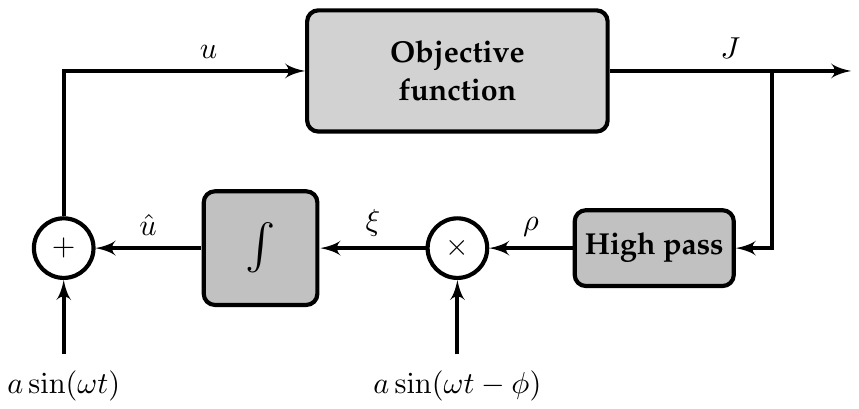
\includegraphics[width=\textwidth]{images/fig_5_21.png}
      \end{figure}
      \vspace{-2mm}
      {\scriptsize\color{gray}
       Fig.~5.21 (p.~202): esquema de la búsqueda de extremos. La
       perturbación sinusoidal se añade a la entrada; el filtro de alta
       frecuencia remueve la media; el $\xi$ resultante estima el gradiente
       y se integra en la entrada optimizadora $\hat{u}$.}
    \end{column}
  \end{columns}
  \fuente
\end{frame}

\begin{frame}{Para profundizar}
  \small
  \textbf{Libros}
  \begin{itemize}
    \item Nocedal \& Wright, \emph{Numerical Optimization} (1999).
    \item Combettes \& Pesquet, \emph{Proximal Splitting Methods in Signal
      Processing} (2011).
    \item Laarhove, Peter \& Aarts, \emph{Simulated Annealing} (1987).
    \item Goldberg, \emph{Genetic Algorithms} (2006).
    \item Koza, Bennett \& Stiffelman, \emph{Genetic Programming as a Darwinian
      Invention Machine} (1999).
  \end{itemize}
  \textbf{Artículos fundacionales}
  \begin{itemize}
    \item Parikh \& Boyd, \emph{Proximal algorithms} (2014).
    \item Zheng, Askham, Brunton, Kutz \& Aravkin, \emph{Sparse relaxed regularized
      regression: SR3}, IEEE Access (2019).
    \item Tropp, \emph{Just relax: Convex programming methods for identifying
      sparse signals in noise} (2006).
    \item Lagarias, Reeds, Wright \& Wright, \emph{Convergence properties of the
      Nelder--Mead simplex method in low dimensions} (1998).
    \item Bertsimas \& Tsitsiklis, \emph{Simulated annealing} (1993).
    \item Kennedy \& Eberhart, \emph{Particle swarm optimization} (1995).
    \item Nedić \& Ozdaglar, \emph{Distributed subgradient methods for
      multi-agent optimization} (2009).
  \end{itemize}
  \vfill
  \centering
  {\footnotesize\color{gray}
    Siguiente capítulo: restricciones y dualidad (ADMM, KKT).}
\end{frame}

\begin{frame}{Ejercicios (del libro, pp.~200--202)}
  \small
  \begin{columns}[T,onlytextwidth]
    \begin{column}{.48\textwidth}
      \textbf{Regresión dispersa (5--1 a 5--7)}
      \begin{itemize}
        \item Comparar LASSO, prox-gradient con $\ell_1$ y $\ell_0$, STLS y
          SR3: con $x\in\R^{10}$ de 2 elementos no nulos y $A$ de $100\times10$
          con ruido $\sim1\%$.
        \item ¿Cuántas iteraciones necesita SR3? ¿Y LASSO?
        \item Repetir con ruido de 1\% a 25\% (5--2).
        \item Graficar error de entrenamiento vs.~número de términos no nulos,
          y superponer el error de prueba (5--3).
        \item Derivar el prox del ridge (5--5) y el de la norma nuclear (5--6).
        \item Reproducir la Fig.~5.4 de Zheng et al.\ (5--7).
      \end{itemize}
    \end{column}
    \begin{column}{.48\textwidth}
      \textbf{Simplex, annealing y enjambre (5--8 a 5--14)}
      \begin{itemize}
        \item Explorar Nelder--Mead sobre los cuatro mínimos con simplex
          iniciales de distintos tamaños (5--8).
        \item Probar distintos calendarios de enfriamiento (5--9).
        \item En $f(x)=\norm{x}_2^2$ y $f(x)=\tfrac12 x^TQx$: variar los
          parámetros del simplex y la dimensión; ¿cuáles son óptimos?
          (5--10)
        \item Repetir con recocido simulado (5--11) y con el punto de silla
          (5--12, 5--13), incluyendo \textbf{momentum} (5--12).
        \item Repetir el punto de silla con PSO (5--14).
      \end{itemize}
      \vspace{1mm}
      \textbf{Otros}: PySR con 3 funciones (5--15) y ruido en Lorenz (5--16);
      \textbf{Extremum seeking} (5--17): perturbación sinusoidal y correlación
      cruzada para estimar el gradiente.
    \end{column}
  \end{columns}
\end{frame}

% =============================================================================
\end{document}
